% Copyright 2021 Joel Feldman, Andrew Rechnitzer and Elyse Yeager, except where noted.
% This work is licensed under a Creative Commons Attribution-NonCommercial-ShareAlike 4.0 International License.
% https://creativecommons.org/licenses/by-nc-sa/4.0/

\begin{frame}{Table of Contents}

\mapofcontentsC{\cf}
\end{frame}

%----------------------------------------------------------------------------------------
%\section{Chapter 3.6: Sketching Graphs}
%----------------------------------------------------------------------------------------
%----------------------------------------------------------------------------------------
\section{3.6.1:  Domain, Intercepts, Asymptotes}
%----------------------------------------------------------------------------------------
%----------------------------------------------------------------------------------------
%----------------------------------------------------------------------------------------


%----------------------------------------------------------------------------------------
\note{It can be very frustrating to learn how to solve a problem only partially, but this is what we do in this section. There are many pieces to curve sketching, and by focusing on one at a time, we teach students how to start sketching before we teach them how to finish sketching. It can be helpful in class to remind students that the remaining pieces are going to be taught soon.}
%----------------------------------------------------------------------------------------
\begin{frame}[t]{Curve Sketching}
\AnswerSpace
\only<1>{\QuestionBar{1}{4}\AnswerYes}
\only<2>{\AnswerBar{1}{4}}
\only<3->{\AnswerNo}
\only<3>{\QuestionBar{2}{4}}
\only<4>{\QuestionBar{3}{4}}
\only<5>{\QuestionBar{4}{4}}
Review: find the domain of the following function.
\[f(x)=\frac{\sqrt{3-x^2}}{\log(x+1)}\]\pause
\answer{\textcolor{M4}{$(-1,0) \cup \left(0,\sqrt{3}\right]$}\pause}

\vfill

Where might you expect $f(x)$ to have a vertical asymptote? What does the function look like nearby?\\
(Recall: a vertical asymptote occurs at $x=a$ if the function has an infinite discontinuity at $a$. That is, $\ds\lim_{x \to a^{\pm}}f(x)=\pm\infty$.)\pause\vfill

Where is $f(x)=0$?\pause\vfill

What happens to $f(x)$ near its other endpoint, $x=-1$?\vfill


\end{frame}
%----------------------------------------------------------------------------------------
\begin{frame}<handout:0>
\centering
\note{Remind students they didn't need to know the graph to answer the previous questions. Rather, questions like those will help them fid the graph later on.}
\begin{tikzpicture}
\myaxis{x}{1}{2}{y}{2}{2}
\draw[C1,thick] plot[domain=0.1:1.73,smooth,yscale=0.1](\x,{sqrt(3-\x*\x)/ln(\x+1)});
\draw[C1, thick] plot[domain=-0.9:-0.1,smooth,yscale=0.1](\x,{sqrt(3-\x*\x)/ln(\x+1)});
\end{tikzpicture}\vfill

%\url{https://www.desmos.com/calculator/9funm5gwrt}
\end{frame}
%----------------------------------------------------------------------------------------%----------------------------------------------------------------------------------------
\begin{frame}{Curve Sketching}
Good things to check:
\begin{itemize}
\item[\textbullet] Domain
\item[\textbullet] Vertical asymptotes: $\displaystyle\lim_{x \rightarrow a} f(x) = \pm\infty$
\item[\textbullet] Intercepts: $x=0$, $f(x)=0$
\item[\textbullet] Horizontal asymptotes and end behavior: $\displaystyle\lim_{x \rightarrow \pm \infty} f(x) $
\end{itemize}\end{frame}
%----------------------------------------------------------------------------------------
%----------------------------------------------------------------------------------------
\begin{frame}[t]{Curve Sketching}
\unote{Example~\eref{text}{eg_3_6_1}}
\AnswerSpace \only<1>{\AnswerYes\QuestionBar{1}{2}}
\only<2>{\AnswerBar{1}{2}}
Identify: domain, vertical asymptotes, intercepts, and horizontal asymptotes

\[f(x) =\frac{x-2}{(x+3)^2}\]

\pause

\vfill
\answer{\color{answercolor}
\begin{itemize}
\item Domain: $x\neq -3$
\item Vertical asymptote: $x=-3$
\item Intercepts: $(2,0)$, $(0,-\frac29)$
\item Horizontal asymptote: $y=0$ in both directions
\end{itemize}\vfill
\url{https://www.desmos.com/calculator/hyzl5cyq7i}}
\note<2>{Graphing takes many steps, and it's often frustrating to see a final result without knowing how to get there. So when I show graphs that we haven't generated in class, I like to add information like: we will learn how to do this part later; look at how the intercepts are where we expect; look at the horizontal asymptotes that we predicted; etc.}
\end{frame}
%----------------------------------------------------------------------------------------
%----------------------------------------------------------------------------------------
\begin{frame}[t]{Curve Sketching}
\AnswerSpace \only<1>{\AnswerYes\QuestionBar{1}{2}}
\only<2>{\AnswerBar{1}{2}}

Identify: domain, vertical asymptotes, intercepts, and horizontal asymptotes
\[f(x) =\frac{(x+2)(x-3)^2}{x(x-5)}\]\pause

\vfill
\answer{\color{answercolor}
\begin{itemize}
\item Domain: $x\neq 0,5$
\item Vertical asymptotes: $x=0$, $x=5$
\item Intercepts: $(-2,0)$, $(3,0)$
\item Horizontal asymptote: none
\end{itemize}\vfill
\url{https://www.desmos.com/calculator/ploa0q7bxn}}
\end{frame}
%----------------------------------------------------------------------------------------
\section*{3.6.2: First Derivative}%: Increasing or Decreasing}
%----------------------------------------------------------------------------------------
\begin{frame}[t]{First Derivative}
\label{eg362usedagain}
\AnswerSpace\unote{Example~\eref{text}{eg sketch simple poly}}
\only<2>{\AnswerYes\QuestionBar{1}{3}}
\only<3-4>{\AnswerBar{1}{3}}

Add complexity: Increasing/decreasing, critical and singular points.\pause

\[f(x)=\frac{1}{2}x^4-\frac{4}{3}x^3-15x^2\]
\only<3|handout:0>{\color{answercolor}
\vfill
\begin{tabular}{p{0.2\textwidth} p{0.8\textwidth}}
\textbf{Domain} & all real numbers\\[1em]
\textbf{Intercepts} & Factor $f(x)=x^2\big(\frac{1}{2}x^2-\frac{4}{3}x-15\big)$. Intercept at the origin; use the quadratic formula to find $x$-intercepts at $x=\frac{4 \pm \sqrt{286}}{3}$, so 
$x \approx 7$ and $x \approx -4.3$.\\[1em]
\raggedright\textbf{End behaviour} & $\dlimx{\infty}f(x) =\infty$\quad and \quad$ \dlimx{-\infty}f(x)=\infty$
\end{tabular}
\vfill
This is the information we've already talked about gathering. Now let's add the first derivative.}
%
\only<4|handout:0>{
\color{answercolor}

\begin{align*}
f'(x)&=2x^3-4x^2-30x\\
&=2x(x^2-2x-15)\\
&=2x(x-5)(x+3)\end{align*} So, critical points are $x=0$, $x=-3$, and $x=5$. No singular points. At the critical points 
$f(0)=0$, $f(-3)=-58.5$, $f(5)=-229.1\overline{6}$. \\[1em]


\vfill\scriptsize\begin{tabular}{c|c|c|c|c|c|c|c|c}\hspace{-5mm}
$x \approx -4.3 $&$x<-3$& x=-3 & $-3<x<0 $& x=0 & $0<x<5$ & x=5&$ x>5$ & $x \approx 7$\\		\hline
\hspace{-5mm}$f(x)=0$&$f'<0$&$CP$&$f'>0$&CP&$f'<0$&CP&$f'>0$&f(x)=0\\	\hline
\hspace{-5mm}intercept&decr&loc min&incr&loc max&decr&loc min&incr&intercept
\end{tabular}
This gives us enough information to draw a skeleton.
}
%
\only<5|handout:0>{
\vfill
\begin{center}
\begin{tikzpicture}[scale=.6]
\myaxis{x}{4.5}{7.5}{}{5}{2.5}

\draw (-4.3,0) node[vertex]{};
\xcoord{-4.3}{-4.3}

\draw (0,0) node[vertex]{};

\draw (7,0) node[vertex]{};
\xcoord{7}{7}

\xcoord{-3}{-3}
\draw (-3,-1.2) node[vertex]{};
\xcoord{5}{5}
\draw (5,-4.6) node[vertex]{};


\draw[dashed] (-5,2)--(-4.3,0)--(-3,-1.2)--(0,0)--(5,-4.6)--(7,0)--(7.5,2);
\end{tikzpicture}
\end{center}

\url{https://www.desmos.com/calculator/lxdlgmhnsl}\vfill}

\end{frame}
%----------------------------------------------------------------------------------------
\begin{frame}[t]
\AnswerSpace
\only<1>{\AnswerYes\QuestionBar{2}{3}}
\only<2-3>{\AnswerBar{2}{3}}
What does the graph of the following function look like?
\[f(x)=\frac{1}{3}x^3+2x^2+4x+24\]\pause\vfill
%
\only<2|handout:0>{\color{answercolor}
\begin{tabular}{p{0.2\textwidth} p{0.8\textwidth}}
\textbf{Domain} &  all real numbers.\\[1em]
\raggedright\textbf{End behaviour} &$\dlimx{-\infty}f(x) = -\infty$ \quad and \quad $\dlimx{\infty}f(x) = \infty$\\[2em]
\textbf{Intercepts} & 
\parbox[t]{.8\textwidth}{
\abovedisplayskip=0pt
\abovedisplayshortskip=0pt
\begin{align*}
f(0)&=24\\
f(x)&=\frac{1}{3}x^2(x+6)+4(x+6)\\
&=\left(\frac{1}{3}x^2+4\right)(x+6)
\end{align*}}
Only two intercepts: $(0,24)$ and $(-6,0)$.
\end{tabular}}
%
\only<3|handout:0>{\color{answercolor}
\begin{tabular}{p{0.2\textwidth} p{0.8\textwidth}}
\textbf{Critical points} & $f'(x)=x^2+4x+4=(x+2)^2$ \quad so $x=-2$ is the location of the only critical point.

$f(-2)=24-\frac83 = 21+\frac13$.
\\[1em]
\textbf{Increasing, decreasing}& $f'(x)>0$ except at $x=-2$, so apart from the critical point, $f(x)$ is increasing
\end{tabular}
\vfill
This is enough for us to draw a skeleton.

}
\only<4|handout:0>{\color{black}
\begin{center}
\begin{tikzpicture}[scale=0.9]
%y scale: 1/8
\myaxis{x}{7}{2}{y}{1.5}{4}
\xcoord{-6}{-6}
\xcoord{-2}{-2}
\ycoord[yshift=1mm]{3}{24}
\draw (-6,0)node[vertex]{};
\draw (-2,2.67)node[vertex]{};
\draw (0,3)node[vertex]{};
\draw[dashed](-7.5,-1.5)--(-7,-.8)--(-2.5,2.67)--(-1.5,2.67)--(.5,3.1)--(1.5,4);;
\end{tikzpicture}
\end{center}
\vfill
\url{https://www.desmos.com/calculator/xum0mstmiv}
}
\vfill
\end{frame}
%----------------------------------------------------------------------------------------
\begin{frame}[t]
\AnswerSpace
\only<1>{\AnswerYes\QuestionBar{3}{3}}
\only<2->{\AnswerBar{3}{3}}

What does the graph of the following function look like?
\[f(x) =e^{\frac{x+1}{x-1}}\]\pause\color{answercolor}\vfill

\only<2|handout:0>{
\begin{tabular}{p{0.2\textwidth} p{0.8\textwidth}}
\textbf{Domain} & $x \neq 1$\\[1em]
\textbf{Vertical asymptotes} & \parbox{.8\textwidth}{\raggedright 
We need to consider what happens as $x$ approaches 1 from the left and the right. 
\begin{align*}
\dlimx{1^-}\frac{x+1}{x-1}&=-\infty &\implies \dlimx{1^-}f(x)&=\displaystyle\lim_{A \rightarrow -\infty}e^A = 0\\
\dlimx{1^+}\frac{x+1}{x-1}&=\infty &\implies \dlimx{1^+}f(x)&=\displaystyle\lim_{A \rightarrow +\infty}e^A = \infty
\end{align*}
}\\[1em]
\raggedright\textbf{End behaviour} & $\displaystyle\lim_{x \rightarrow \pm\infty} \frac{x+1}{x-1}=1$,
so $\displaystyle\lim_{x \rightarrow \pm\infty} f(x) = e$\\[2em]
\textbf{Intercepts} & $f(0)=\frac{1}{e}$; there are no roots
\end{tabular}
}
%
\only<3|handout:0>{
\begin{tabular}{p{0.2\textwidth} p{0.8\textwidth}}
\textbf{Critical points} & $f'(x)=e^{\frac{x+1}{x-1}}\left( \frac{-2}{(x-1)^2}\right)$ \qquad no critical points
\\[2em]
\textbf{Increasing, decreasing} & 
$f(x)$ is decreasing everywhere it is defined
\end{tabular}
\vfill
This information is enough to draw a skeleton.
}
%
\only<4|handout:0>{
\begin{center}
\begin{tikzpicture}[xscale=0.5]
\myaxis{x}{10}{10}{y}{0}{4}
\draw[dashed] (-10,2.6)--(-5,2.21)--(1,0);
\draw[dashed] (10,2.6)--(2,2.7)--(1,4);
\xcoord{1}{1}
\ycoord{2.72}{e}
\ycoord{0.37}{\frac1e}
\draw (0,0.37)node[vertex]{};
\draw (1,0)node[opendot]{};

\end{tikzpicture}
\end{center}
\vfill
\url{https://www.desmos.com/calculator/x0cccy1ggj}
}
\end{frame}
%----------------------------------------------------------------------------------------
%----------------------------------------------------------------------------------------

\begin{frame}[t]{Signs of Factored Functions \hfill\only<beamer>{\hyperlink{signchangesend}{\beamerskipbutton{skip sign changes}}}}
\note<1>{Students often learned in high school that they should test points between consecutive roots, which is much slower.}

\begin{center}
	\begin{tabular}{lcccl}
		$f(x)=$&\color{C1}$\alert<2>{(x-1)}$&
		\color{C1}$(x-2)$\only<27->{$^2$}&
		\color{C1}$(x-3)$&
		\iftoggle{printsolutions}{
			\\	&	\only<2,9-13,29>{\alert{$-$}}
			\only<3,14-24,30-31>{\textcolor{C1}{$+$}}
			&	\only<4,9-18>{\alert{$-$}}
			\only<5,19-24,28->{\textcolor{C1}{$+$}}
			&	\only<6,9-23,29-30>{\alert{$-$}}
			\only<7,24,31->{\textcolor{C1}{$+$}}}{}
	\end{tabular}
	\vfill
	\begin{tikzpicture}
	\draw[thick, <->](-1,0)--(10,0) node[right]{$x$};
	\iftoggle{printsolutions}{
		\foreach \x in {1,2,3}{
			\xcoord{3*\x}{\x}
			\onslide<8-25>{\draw (3*\x,.75) node{
\includegraphics[width=1cm]{Clipart/switch2.png}};
			\index{
\includegraphics[height=5mm]{Clipart/switch2.png} 
			\href{https://thenounproject.com/icon/1823877/}{`switch'} by
			\href{https://thenounproject.com/Vntole/}{Anthony Ledoux} is licensed under
			\CCBYthree~
			(accessed 3 Oct 2018)}
			}
			\MULTIPLY{2}{\x}{\s}
			\ADD{1}{\s}{\t}
			\MULTIPLY{3}{\x}{\x}
			\onslide<\s>{\draw[line width=3pt, M4](-.5,0)--(\x,0)node[opendot]{};} 
			\onslide<\t>{\draw[line width=3pt, C1](\x,0) node[opendot]{}--(10,0); }}
		\foreach \l in {0,1,2}{
			\foreach \x in {1,...,5}{
				\DIVIDE{\x}{2}{\step}
				\MULTIPLY{3}{\l}{\xc}
				\ADD{\xc}{\step}{\xc}
				\MULTIPLY{\l}{5}{\s}
				\ADD{\s}{8}{\s}
				\ADD{\s}{\x}{\s}
				\onslide<\s>{\draw(\xc,0)node[vertex, label=below:{$x$}]{};}
			}
		}
		\onslide<24>{\draw (9.5,0)node[vertex, label=below:{$x$}]{};}
		\onslide<26>{
			\draw[ultra thick, <->, opacity=0.75, C1] (-1,-1)--(3,-1) node[midway, below]{negative};	
			\draw[ultra thick, <->, opacity=0.75, M4] (3,1)--(6,1) node[midway, above]{positive};	
			\draw[ultra thick, <->, opacity=0.75, C1] (6,-1)--(9,-1) node[midway, below]{negative};	
			\draw[ultra thick, <->, opacity=0.75, M4] (9,1)--(10,1) node[midway, above]{positive};	
		}
		\onslide<29>{\draw[line width=3pt, C1] (-.5,0)--(3,0) node[opendot]{};}
		\onslide<30>{\draw[line width=3pt, M4] (3,0) node[opendot]{}--(9,0) node[opendot]{};}
		\onslide<31>{\draw[line width=3pt, C1] (9,0) node[opendot]{}--(9.8,0);}
		\onslide<28->{
			\draw(3,.75) node{
\includegraphics[width=1cm]{Clipart/switch2.png}};
			\draw(9,.75) node{
\includegraphics[width=1cm]{Clipart/switch2.png}};
			\index{
\includegraphics[height=5mm]{Clipart/switch2.png} 
			\href{https://thenounproject.com/icon/1823877/}{`switch'} by
			\href{https://thenounproject.com/Vntole/}{Anthony Ledoux} is licensed under
			\CCBYthree~
			(accessed 3 Oct 2018)}
			}
	}{}
	\end{tikzpicture}
\end{center}
\vfill
\iftoggle{printsolutions}{ \onslide<8->{Sign of entire function:}
	\only<9-13,19-23>{\alert{\Huge\colorbox{C1!20}{$\mathbf{-}$}}}
	\only<14-18,24>{\textcolor{C1}{\Huge\colorbox{M4!20}{$\mathbf{+}$}}}
}{}
\StatusBar{1}{31}
\end{frame}
%-------------------------------------------------------------
%-------------------------------------------------------------
\begin{frame}[t]{Signs of Factored Functions \hfill\only<beamer>{\hyperlink{signchangesend}{\beamerskipbutton{skip sign changes}}}}

\[f(x) = (x-3)(x-1)^2x(x+2)^3(x+5)^4\]
\textcolor{green}{Where is $f(x)$ positive? Where is it negative?}
\vfill
\begin{center}
	\begin{tikzpicture}
	\draw[thick, <->] (-6,0)--(6,0);
	\foreach \x in {-5,...,5}{\xcoord{\x}{\x}};
	\iftoggle{printsolutions}{\onslide<2->{{\foreach \x in {3,0,-2}{\draw (\x,-.5) node[shape=rectangle, white, fill=black]{$\x$}; }}}
		\onslide<3->{\color{C1} \draw[thick, <->] (-6,-1.5)--(-2,-1.5) node[midway, below]{negative};
			\draw (-5,-1.5) node{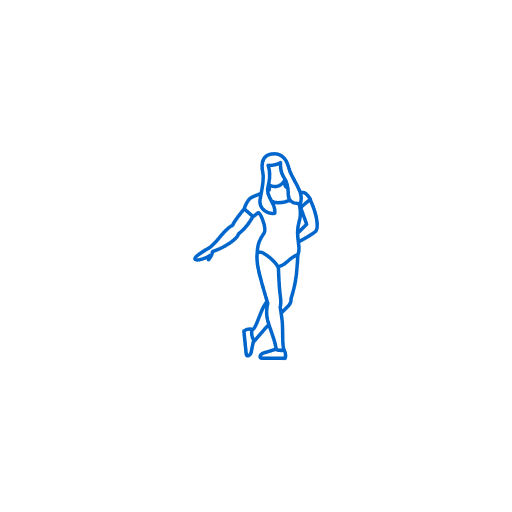
\includegraphics[width=2cm]{Clipart/negative1.png}};
			\index{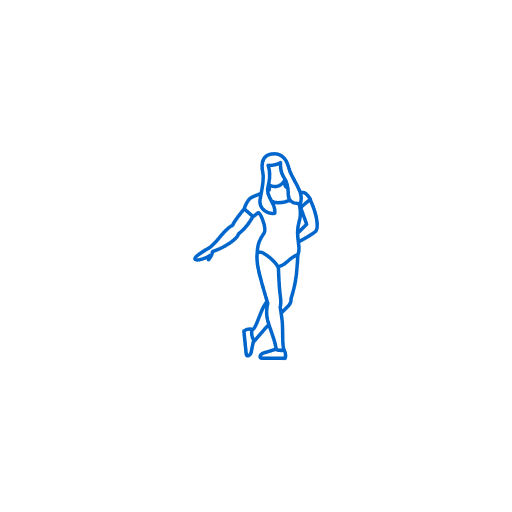
\includegraphics[height=1cm]{Clipart/negative1.png}
			\href{https://thenounproject.com/icon/1298614/}{`Dancer'} by
			\href{https://thenounproject.com/thepyramidschool/}{The Pyramid School}
			is licensed under \CCBYthree
			~ (accessed Oct 2018)}
		}
		\onslide<4->{\color{M4} \draw[thick, <->] (-2,1)--(0,1) node[midway, below]{positive};
			\draw (-1.5,1.6) node{
\includegraphics[width=2cm]{Clipart/positive2.png}};
			\index{
\includegraphics[height=7mm]{Clipart/positive2.png} 
			\href{https://thenounproject.com/icon/623418/}{`dance'} by
			\href{https://thenounproject.com/EvgeniMoryakov/}{Evgeni Moryakov}
			is licensed under \CCBYthree~
			(accessed 3 Oct 2018)}
			}
		\onslide<5->{\color{C1} \draw[thick, <->] (0,-1.5)--(3,-1.5) node[midway, below]{negative};
			\draw (1,-1.1) node{
\includegraphics[width=1.25cm]{Clipart/negative2.png}};
			\index{
\includegraphics[height=7mm]{Clipart/negative2.png} 
			\href{https://thenounproject.com/icon/11089/}{`Dancer'}
			by
			\href{https://thenounproject.com/jmkeuning/}{James Keuning} is in the public domain
			(accessed 3 Oct 2018) }}
		\onslide<6->{\color{M4} \draw[thick, <->] (3,1)--(6,1) node[midway, below]{positive};
			\draw (4,1.5) node{
\includegraphics[width=1.5cm]{Clipart/positive1.png}};
			\index{
\includegraphics[height=7mm]{Clipart/positive1.png} 
			\href{https://thenounproject.com/icon/12712/}{`Dancer'}
			by
			\href{https://thenounproject.com/2moriah/}{Moriah Rich}
			is licensed under
			\CCBYthree~
			(accessed 3 Oct 2018)}}
			}{}
	\end{tikzpicture}
\end{center}
\StatusBar{1}{6}
\end{frame}
%-------------------------------------------------------------

\section*{3.6.3: Concavity}
%----------------------------------------------------------------------------------------

%----------------------------------------------------------------------------------------

%----------------------------------------------------------------------------------------
\begin{frame}{Concavity}\label{signchangesend}
\unote{Definition~\eref{text}{def_3_6_1}}
\begin{multicols}{2}
\begin{tikzpicture}
\myaxis{x}{2}{2}{y}{1.2}{3.2}
\draw[ultra thick, C1] plot[domain=-2:2,smooth](\x,{(\x*\x-1)});

\draw[ultra thick, M4] plot[domain=-2:-1,smooth](\x,{1.25-4.5-3*\x});
\draw (-1.5,1.25) node[M4, vertex]{};
\draw[ultra thick, M4] plot[domain=-.5:.5,smooth](\x,{-1});
\draw (0,-1) node[M4, vertex]{};
\draw[ultra thick, M4] plot[domain=1:2,smooth](\x, {1.25-4.5+3*\x});
\draw (1.5,1.25) node[M4, vertex]{};
\end{tikzpicture}
\begin{itemize}
\item Slopes are increasing
\item $f''(x)>0$
\item ``concave up''
\item tangent line below curve
\end{itemize}
\columnbreak

\begin{tikzpicture}
\myaxis{x}{2}{2}{y}{1.2}{3.2}
\draw[ultra thick, C1] plot[domain=-2:2,smooth](\x,{(-\x*\x+3)});
\draw[ultra thick, M4] plot[domain=-2:-1,smooth](\x,{3/4+3*(\x+1.5)});
\draw (-1.5,3/4) node[M4, vertex]{};
\draw[ultra thick, M4] plot[domain=-.5:.5,smooth](\x,{3});
\draw (0,3) node[M4, vertex]{};
\draw[ultra thick, M4] plot[domain=1:2,smooth](\x, {3/4-3*(\x-1.5)});
\draw (1.5,3/4) node[M4, vertex]{};
\end{tikzpicture}
\begin{itemize}
\item Slopes are decreasing
\item $f''(x)<0$
\item ``concave down''
\item tangent line above curve
\end{itemize}

\end{multicols}
\end{frame}
%----------------------------------------------------------------------------------------
%----------------------------------------------------------------------------------------
\begin{frame}{Mnemonic}
\begin{center}
\begin{tikzpicture}	
\draw[M4] (-1,1) node{$+$};
\draw[M4] (1,1) node{$+$};
\draw[M4, ultra thick] (-1,0) to[out=-45, in=-135] (1,0);
\end{tikzpicture}
\hspace{2cm}
\begin{tikzpicture}	
\draw[M4] (-1,1) node{$-$};
\draw[M4] (1,1) node{$-$};
\draw[M4, ultra thick] (-1,-.5) to[out=45, in=135] (1,-.5);
\end{tikzpicture}
\end{center}
\end{frame}
%----------------------------------------------------------------------------------------

%----------------------------------------------------------------------------------------
\begin{frame}{Concavity}
\unote{Definition~\eref{text}{def_3_6_1}}
\note<1>{``Just by staring at it, decide where this function is concave up, and where it is concave down."}
\begin{tikzpicture}[yscale=0.8]

\draw[ultra thick, C1] plot[domain=-2:.5,smooth](\x,{\x*\x});
\draw[ultra thick, C1] plot[domain=.5:6.28,smooth](\x-.02,{sin(\x r)-.25});
\draw[ultra thick, C1] plot[domain=6.25:8,smooth](\x,{(\x-5.75)*(\x-5.78)-.5});

\answer{
\onslide<2->{\draw[thick, M4, <->] (-2,-2.5)--(0.5,-2.5);
\draw[M4] (-.75,-3) node{concave up}; }
\onslide<2>{\draw[dashed, M4, pattern=north east lines, pattern color=M4] (-2,-2.5)--(-2,4)--(.5,4)--(.5,-2.5);}

\onslide<3->{\draw[thick, M3, <->] (.5,-2.5)--(3.16,-2.5);
\draw[M3] (1.75,-3) node{concave down}; }
\onslide<3>{\draw[dashed, M3, pattern=north west lines, pattern color=M3] (3.16,-2.5)--(3.16,4)--(.5,4)--(.5,-2.5);}

\onslide<4->{\draw[thick, M4, <->] (3.16,-2.5)--(8,-2.5);
\draw[M4] (5,-3) node{concave up}; }
\onslide<4>{\draw[dashed, M4, pattern=north east lines, pattern color=M4] (3.16,-2.5)--(3.16,4.5)--(8,4.5)--(8,-2.5);}

\onslide<5->{\draw (.5,.25) node[vertex](a){};
\draw (3.16,-.25) node[vertex](b){};
}

\onslide<6->{
\draw[<-] (a)--(.5,-.75) node[below]{inflection point};
\draw[<-] (b)--(3.17,.75) node[above]{inflection point};}

\onslide<7->{
\draw (.5,-1.25) node[below]{$f''(x)$ changes sign};}
}%answer
\end{tikzpicture}
\end{frame}
%----------------------------------------------------------------------------------------
%---------------------------------
\begin{frame}
\note<1>{It is a very common misconception that e.g. concave up functions are also increasing. Be wary of conflating first and second derivatives.}
Sketch graphs with the following properties, or explain that none exist.
\vfill
\begin{tabular}{|c|c|c|}
	\hline
	&concave up & concave down\\
	\hline
	increasing & \parbox{4cm}{
		\begin{tikzpicture}[scale=0.9]
		\myaxis{x}{2}{2}{y}{1}{1}
		\iftoggle{printsolutions}{
			\onslide<2->{\draw[thick, C4] plot[domain=-2:2, smooth](\x,{1.5^\x-1.25});}
		}{}
		
		\end{tikzpicture}	
	} & \parbox{4cm}{
		\begin{tikzpicture}[scale=0.9]
		\myaxis{x}{2}{2}{y}{1}{1}
		\iftoggle{printsolutions}{
			\onslide<3->{\draw[thick, C4] plot[domain=-2:2, smooth](\x,{sqrt(\x+2.1)-1});}
		}{}
		\end{tikzpicture}	
	}\\
	\hline	decreasing & \parbox{4cm}{
		\begin{tikzpicture}[scale=0.9]
		\myaxis{x}{2}{2}{y}{1}{1}
		\iftoggle{printsolutions}{
			\onslide<4->{\draw[thick, C4] plot[domain=-2:2, smooth](\x,{1.25-sqrt(\x+2.1)});}
		}{}
		
		\end{tikzpicture}	
	} & \parbox{4cm}{
		\begin{tikzpicture}[scale=0.9]
		\myaxis{x}{2}{2}{y}{1}{1}
		\iftoggle{printsolutions}{
			\onslide<5->{\draw[thick, C4] plot[domain=-2:2, smooth](\x,{1.5-1.5^\x});}
		}{}
		
		\end{tikzpicture}	
	}\\
	\hline
\end{tabular}


\end{frame}
%---------------------------------
%----------------------------------------------------------------------------------------
\begin{frame}[t]{Poll Questions}
Describe the concavity of the function $f(x)=e^x$.
\begin{enumerate}[A.]
\alert<2-|handout:0>{\item  concave up}
\item  concave down
\item  concave up for $x<0$; concave down for $x>0$
\item  concave down for $x<0$; concave up for $x>0$
\item  I'm not sure
\end{enumerate}

\onslide<3->{Is it possible to be concave up and decreasing?
\begin{center}
\hfill \alert<4-|handout:0>{A. Yes} \hfill
B. No \hfill
C. I'm not sure \hfill~
\end{center}}

\onslide<5->{Suppose a function $f(x)$ is defined for all real numbers, and is concave up on the interval $[0,1]$. Which of the following must be true?
\begin{enumerate}[A.]
\alert<6-|handout:0>{\item  $f'(0)<f'(1)$}
\item  $f'(0)>f'(1)$
\item  $f'(0)$ is positive
\item  $f'(0)$ is negative
\item  I'm not sure
\end{enumerate}}

\only<1>{\QuestionBar{1}{3}\AnswerYes}
\only<2>{\AnswerBar{1}{3}}
\only<3>{\QuestionBar{2}{3}\AnswerYes}
\only<4>{\AnswerBar{2}{3}}
\only<5>{\QuestionBar{3}{3}\AnswerYes}
\only<6>{\AnswerBar{3}{3}}
\end{frame}
%----------------------------------------------------------------------------------------
%---------------------------------

%----------------------------------------------------------------------------------------
\begin{frame}[t]{Revisiting a previous example}
\AnswerSpace
\only<1-2>{\AnswerYes\QuestionBar{1}{2}}
\only<3->{\AnswerBar{1}{2}}
\note<1>{Rather than start from scratch, here's an example we already have a skeleton for. The second derivative factors nicely, so we can quickly see how to add concavity to our sketches.}
\hfill\hyperlink{eg362usedagain}{\beamerreturnbutton{original example}}
\unote{Example~\eref{text}{eg_3_6_2}}
\[f(x)=\frac{1}{2}x^4-\frac{4}{3}x^3-15x^2\]

\vfill
\begin{center}
\begin{tikzpicture}[scale=.5]
\myaxis{x}{4.5}{7.5}{y}{5}{2.5}

\draw (-4.3,0) node[vertex]{};
\draw (-4.3,.2)--(-4.3,-.2) node[below]{-4.3};

\draw (0,0) node[vertex]{};

\draw (7,0) node[vertex]{};
\draw (7,.2)--(7,-.2) node[below]{7};

\draw (-3,.2)--(-3,-.2) node[below]{-3};
\draw (-3,-1.2) node[vertex]{};
\draw (-.2,-1.2)--(.2,-1.2) node[right]{$-58.5$};

\draw (5,.2)--(5,-.2) node[below]{5};
\draw (5,-4.6) node[vertex]{};
\draw (.2,-4.6)--(-.2,-4.6) node[left]{$-229.1\overline{6}$};

\onslide<-3>{
\draw[dashed] (-5,2)--(-4.3,0)--(-3,-1.2)--(0,0)--(5,-4.6)--(7,0)--(7.5,2);
}

\onslide<3-|handout:0>{\color{M4}
\draw (3,.2)--(3,-.2) node[below]{3};
\draw (-1.7,.2)--(-1.7,-.2) node[below]{$-\frac{5}{3}$};}

\onslide<4-|handout:0>{\color{C1}
\draw[ultra thick] plot[domain=-4.6:7.2, samples=100]
(\x,{(pow(\x,4)/2-4*pow(\x,3)/3-15*\x*\x)*.02});}
\end{tikzpicture}
\end{center}\vfill
\pause\color{M4}
$f''(x)=6x^2-8x-30 = 2(x-3)(3x+5)$
\end{frame}

%----------------------------------------------------------------------------------------
\begin{frame}[t]
\AnswerSpace
\only<1>{\AnswerYes\AnswerBar{2}{2}}
\only<2->{\QuestionBar{2}{2}}
Sketch:\[f(x)=x^5-15x^3\]

\note<1>{Mention symmetry, to motivate next subsection.}\vfill

\only<2|handout:0>{
\color{answercolor}
\begin{tabular}{p{0.2\textwidth} p{0.8\textwidth}}
\textbf{Domain}  & Defined and differentiable for all real numbers.\\[1em]
\textbf{Intercepts} & \parbox[t]{.8\textwidth}{$f(x) = x^3(x^2-15)$:\\ Roots are at $x=0$ and $x=\pm \sqrt{15} \approx \pm 4$}\\[2em]
\raggedright
\textbf{End behaviour} & $\dlimx{-\infty}f(x)=-\infty$ and  $\dlimx{\infty}f(x)=\infty$ 
\\[2em]
\textbf{Critical points} & $f'(x)=5x^4-45x^2=5x^2\big(x^2-9\big)$. So the critical points are $x=0$, $x=\pm 3$.
\\[1em]
\textbf{Increasing, decreasing} & Increasing on $(-\infty,-3)$, decreasing on $(-3,0)$ and $(0,3)$, increasing on $(3,\infty)$\\[1em]
\raggedright\textbf{Local extrema} & From intervals of increase and decrease: local max at $x=-3$ and local min at $x=3$
\end{tabular}
}
\only<3|handout:0>{
\color{answercolor}
\begin{tabular}{p{0.2\textwidth} p{0.8\textwidth}}
\textbf{Concavity} & $f''(x)=20x^3-90x=10x(2x^2-9)=0$ for $x=0$ and 
 $x=\pm\frac{3}{\sqrt{2}} \approx \pm 2$. All of these are inflection points; concave down $(-\infty, -\frac{3}{\sqrt 2})$, concave up $(-\frac{3}{\sqrt{2}},0)$, concave down $(0,\frac{3}{\sqrt 2})$, and concave up $(\frac{3}{\sqrt{2}},\infty)$.\\[1em]
\raggedright\textbf{$y$-values of notable points} & $f(3)=-162$, $f(-3)=162$, $f(-3/\sqrt{2})\approx 100$, $f(3/\sqrt{2})\approx -100$
\end{tabular}
}

\only<4-|handout:0>{
\begin{center}
\begin{tikzpicture}
%yscale: 1/100
\myaxis{x}{5}{5}{y}{3}{3}
\xcoord{3}{3}
\xcoord{-3}{-3}
\xcoord{2.12}{\frac{3}{\sqrt 2}}
\xcoord{-2.12}{-\frac{3}{\sqrt 2}}
\ycoord{1.62}{162}
\ycoord{-1.62}{-162}
\xcoord{3.87}{\sqrt 15}
\xcoord{-3.87}{-\sqrt 15}
\draw (0,0)node[vertex]{};
\draw (0,0)node{\huge $-$};
\foreach \r in {0,180}{
	\begin{scope}[rotate=\r]
		\draw (3.87,0)node[vertex](c){};
		\draw (3,-1.62)node[vertex]{};
		\draw (2.8,-1.62)coordinate(b1){};
		\draw (3.2,-1.62)coordinate(b2){};
		\draw (3,-1.62)node{\huge $-$};
		\draw (2.12,-1)node[vertex](a){};
		\only<5>{\draw[dashed] (0.2,0)--(a)--(b1)--(b2)--(c)--(5,3);}
		\only<6>{\draw[C1,thick] plot[domain=0:4.2,smooth](\x,{(\x*\x*\x*\x*\x-15*\x*\x*\x)/100});}
	\end{scope}}
\end{tikzpicture}
\vfill
\only<6>{\url{https://www.desmos.com/calculator/uoii6nmgr8}}
\end{center}}

\end{frame}
%----------------------------------------------------------------------------------------
%----------------------------------------------------------------------------------------
\section*{3.6.4 : Symmetries}
%----------------------------------------------------------------------------------------
%----------------------------------------------------------------------------------------
%----------------------------------------------------------------------------------------
\begin{frame}{Even and Odd Functions}
\begin{center}
\begin{tikzpicture}[scale=.6]
\myaxis{x}{5}{5}{y}{2}{2}
{\color{C1}
\only<1-2|handout:1>{\draw[ultra thick] plot[domain=-4:4, samples=50]
(\x,{(pow(\x,5)-15*pow(\x,3))*.02});}}
{\color{C1}
\only<3-4|handout:2>{\draw[ultra thick] plot[domain=-4:0, samples=50]
(\x,{(pow(\x,5)-15*pow(\x,3))*.02});
\draw[ultra thick] plot[domain=0:4, samples=50]
(\x,{-(pow(\x,5)-15*pow(\x,3))*.02});}}
\end{tikzpicture}

\onslide<1-2|handout:0>{$f(x)=x^5-15x^3$}

\onslide<2,4|handout:0>{\textcolor{M3}{\only<2>{odd}\only<4>{even} function }}
\end{center}

\end{frame}
%----------------------------------------------------------------------------------------
%----------------------------------------------------------------------------------------
\begin{frame}[t]

\begin{block}{Even Function -- Definition~\eref{text}{def:APPeven}}
A function $f(x)$ is \textcolor{M3}{even} if, for all $x$ in its domain,
\[f(-x)=f(x)\]
\end{block}\vfill

\begin{tikzpicture}[xscale=.7,yscale=0.5]
\myaxis{x}{6.3}{6.3}{y}{2}{2}
\draw[ultra thick, C1] plot[domain=-6.3:6.4, samples=100]
(\x,{2*cos(\x r)}) node[above]{$y=f(x)$};

\onslide<2-|handout:0>{\draw[C1] (3.1,-2) node[vertex](a){};
\draw[C1] (a) node[below]{$(3,-1)$};}
\onslide<4-|handout:0>{\draw[C1] (-3.1,-2) node[vertex](-a){};
\draw[C1] (-a) node[below]{$(-3,-1)$};}

\onslide<5-|handout:0>{\draw[C1] (6.28,2) node[vertex](b){};
\draw[C1] (b) node[below right]{$(6,1)$};}
\onslide<7-|handout:0>{\draw[C1] (-6.28,2) node[vertex](-b){};
\draw[C1] (-b) node[below left]{$(-6,1)$};}
\end{tikzpicture}
\pause\vfill

\answer{Suppose $f(3)=-1$. \pause Then $f(-3)=$ \pause $-1$ also.\pause

Suppose $f(6)=1$. \pause Then $f(-6)=$ \pause $1$ also.}
\end{frame}
%----------------------------------------------------------------------------------------
%----------------------------------------------------------------------------------------
\begin{frame}[t]{Even Functions}
\begin{block}{Even Function -- Definition~\eref{text}{def:APPeven}}
A function $f(x)$ is \textcolor{M3}{even} if, for all $x$ in its domain,
\[f(-x)=f(x)\]
\end{block}
Examples:\\\pause
$f(x)=x^2$\\\pause
$f(x)=x^4$\\ \pause
$f(x)=\cos(x)$\\ \pause
$f(x)=\dfrac{x^4+\cos(x)}{x^{16}+7}$
\end{frame}
%----------------------------------------------------------------------------------------
%----------------------------------------------------------------------------------------
\begin{frame}[t]{Odd Functions}

\begin{tikzpicture}[xscale=.7,yscale=0.5]
\myaxis{x}{6.3}{6.3}{y}{2}{2}

\draw[ultra thick, C1] plot[domain=-6.3:6.4, samples=100]
(\x,{2*sin(\x r)}) node[above]{$y=f(x)$};

\answer{
\onslide<2->{\draw[C1] (1.6,2) node[vertex](a){};
\draw[C1] (a) node[above]{$(1,2)$};}
\onslide<4->{\draw[C1] (-1.6,-2) node[vertex](-a){};
\draw[C1] (-a) node[below]{$(-1,-2)$};}

\onslide<5->{\draw[C1] (4.7,-2) node[vertex](b){};
\draw[C1] (b) node[below]{$(3,-2)$};}
\onslide<7->{\draw[C1] (-4.7,2) node[vertex](-b){};
\draw[C1] (-b) node[above]{$(-3,2)$};}
}%answer
\end{tikzpicture}
\pause\vfill

Suppose $f(1)=2$. \pause Then $f(-1)=$\pause \answer{$-2$.}\pause

Suppose $f(3)=-2$. \pause Then $f(-3)=$\pause \answer{$2$.}\pause\vfill

\begin{block}{Odd Function -- Definition~\eref{text}{def:APPodd}}
A function $f(x)$ is \textcolor{M3}{odd} if, for all $x$ in its domain,\pause
\[f(-x)=-f(x)\]
\end{block}
\end{frame}
%----------------------------------------------------------------------------------------
%----------------------------------------------------------------------------------------
\begin{frame}[t]{Odd Functions}
\begin{block}{Odd Function -- Definition~\eref{text}{def:APPodd}}
A function $f(x)$ is \textcolor{M3}{odd} if, for all $x$ in its domain,
\[f(-x)=-f(x)\]
\end{block}
Examples:\\\pause
$f(x)=x$\\\pause
$f(x)=x^3$\\ \pause
$f(x)=\sin(x)$\\ \pause
$f(x)=\dfrac{x(1+x^2)}{x^2+5}$
\end{frame}
%----------------------------------------------------------------------------------------
%----------------------------------------------------------------------------------------
\begin{frame}[t]{Poll Tiiime}
\only<1>{\QuestionBar{1}{5}\AnswerYes}
\only<2>{\AnswerBar{1}{5}}
\only<3>{\QuestionBar{2}{5}\AnswerYes}
\only<4>{\AnswerBar{2}{5}}
Pick out the \only<1-2|handout:1>{\textcolor{M3}{odd}}\only<3-4|handout:2>{\textcolor{M3}{even}} function.
\vfill
\begin{center}
A: \begin{tikzpicture}[scale=.3]
\myaxis{x}{3}{3}{y}{3}{3}
\draw[C1, ultra thick] plot[domain=-3:3,smooth](\x,{.15*exp(\x)});
\end{tikzpicture}
\hspace{2cm}
\alert<4|handout:0>{B}: \begin{tikzpicture}[scale=.3]
\myaxis{x}{3}{3}{y}{3}{3}\draw[C1, ultra thick] plot[domain=-3:3,smooth](\x,{2*(\x*\x)/3-3});
\end{tikzpicture}

\vfill
\alert<2|handout:0>{C}: \begin{tikzpicture}[scale=.3]
\myaxis{x}{3}{3}{y}{3}{3}\draw[C1, ultra thick] (-3,-3)--(-1.5,-3)--(1.5,3)--(3,3);
\end{tikzpicture}
\hspace{2cm}
D: \begin{tikzpicture}[scale=.3]
\myaxis{x}{3}{3}{y}{3}{3}\draw[C1, ultra thick] plot[domain=-1:3,smooth](\x,{\x*(\x-2)});
\end{tikzpicture}
\end{center}
\vfill
\end{frame}
%----------------------------------------------------------------------------------------
%----------------------------------------------------------------------------------------
\begin{frame}[t]{Even more Poll tiiiiime}
\only<1>{\QuestionBar{3}{5}\AnswerYes}
\only<2>{\AnswerBar{3}{5}}

Suppose $f(x)$ is an \textcolor{M3}{odd} function, continuous, defined for all real numbers. What is $f(0)$? Pick the best answer.
\begin{enumerate}[A.]
\item $f(0)=f(-0)$ \onslide<3-|handout:0>{\textcolor{answercolor}{$\leftarrow$ true but uninteresting, for all functions}}
\item $f(0)=-f(0)$ \onslide<4-|handout:0>{\textcolor{answercolor}{$\leftarrow$ only possible for $f(0)=0$}}
\item $f(0)=0$ \onslide<5-|handout:0>{\textcolor{answercolor}{$\leftarrow$ this is equivalent to the choice above}}
\alert<2-|handout:0>{\item all of the above are true}
\item none of the above are necessarily true
\end{enumerate}
\end{frame}
%----------------------------------------------------------------------------------------
%----------------------------------------------------------------------------------------
\begin{frame}[t]{Even more and more Poll tiiiiime}
\only<1>{\QuestionBar{4}{5}\AnswerYes}
\only<2>{\AnswerBar{4}{5}}

Suppose $f(x)$ is an \textcolor{M4}{even} function, continuous, defined for all real numbers. What is $f(0)$? Pick the best answer.
\begin{enumerate}[A.]
\alert<2|handout:0>{\item $f(0)=f(-0)$ }
\item $f(0)=-f(0)$ 
\item $f(0)=0$ 
{\item all of the above are true}
{\item none of the above are necessarily true}
\end{enumerate}
\end{frame}
%----------------------------------------------------------------------------------------
%----------------------------------------------------------------------------------------
\begin{frame}[t]{OK OK... last one}
\only<1>{\QuestionBar{5}{5}\AnswerYes}
\only<2>{\AnswerBar{5}{5}}

Suppose $f(x)$ is an \textcolor{M4}{even} function, differentiable for all real numbers. What can we say about $f'(x)$?
\begin{enumerate}[A.]
\item $f'(x)$ is also even 
\alert<2|handout:0>{\item $f'(x)$ is odd }
\item $f'(x)$ is constant 
\item all of the above are true
\item none of the above are necessarily true
\end{enumerate}

\end{frame}
%----------------------------------------------------------------------------------------

%----------------------------------------------------------------------------------------
%----------------------------------------------------------------------------------------
\begin{frame}[t]{Periodicity}
\begin{block}{Periodic -- Definition~\eref{text}{def:APPperiodic}}
A function is \textcolor{M3}{periodic} with period $P>0$ if
\[f(x)=f(x+P)\]
whenever $x$ and $x+P$ are in the domain of $f$, and $P$ is the smallest such (positive) number
\end{block}
Examples: $\sin (x)$, $\cos (x)$ both have period $2\pi$;\quad $\tan (x)$ has period $\pi$.
\end{frame}
%----------------------------------------------------------------------------------------
%----------------------------------------------------------------------------------------
\begin{frame}[t]\MoreSpace\AnswerYes

Ignoring concavity, sketch $f(x)=\sin(\sin x)$.

\vfill

Challenge: ignoring exact locations of extrema, sketch $g(x)=\sin(2\pi \sin x)$.

\vfill
\note{The second one really is quite tough; you can let the faster students work on it while the rest of the class is working on $f(x)$. Then the solution is more-or-less in the slides if they want to look, with no need to do it in class.}
\end{frame}
%----------------------------------------------------------------------------------------
\begin{frame}<handout:0>[t]
\[f(x)=\sin(\sin x)\]\pause
\AnswerBar{1}{2}
\color{answercolor}
Sin is periodic; since $\sin x = \sin (2\pi+x)$, then $\sin(\sin x) = \sin (\sin (2\pi+x))$, so $f(x)$ is also periodic. It suffices to sketch $f(x)$ for an interval of length $2\pi$, because any such segment will repeat.

Since the function is also odd, if we sketch it on the interval $[0,\pi]$, then we can extrapolate to the interval $[-\pi,0]$. So we consider the interval $[0,\pi]$.

\begin{itemize}
\item Intercepts: $(0,0)$, $(0,\pi)$
\item First derivative: $f'(x) = \cos(\sin x)\cdot \cos(x)$ 
	\begin{itemize}
        \item For $0\le x\le\pi$, we have $0\le\sin x\le 1<\frac{\pi}{2}$ 
            and hence $0<\cos(\sin x)\le 1$.
	\item CP: $x= \frac\pi2$
	\item increasing: $(0,\pi/2)$
	\item decreasing: $(\pi/2,0)$
	\end{itemize}
\end{itemize}
\end{frame}
%----------------------------------------------------------------------------------------
\begin{frame}<handout:0>
\AnswerBar{1}{2}
\color{answercolor}
\begin{multicols}{2}
\begin{enumerate}
\item Interval $(0,\pi)$ skeleton, based on above work:

\begin{tikzpicture}
\myaxis{x}{0}{3.5}{y}{0}{1}
\color{C1}
\draw (0,0)node[vertex]{};
\draw (3.14,0)node[vertex]{};
\draw[dashed] (0,0)--(1.57,1)--(3.14,0);
\xcoord{3.14}{\pi}
\end{tikzpicture}

\item Make into a smooth curve:

\begin{tikzpicture}
\myaxis{x}{0}{3.5}{y}{0}{1}
\color{C1}
\draw (0,0)node[vertex]{};
\draw (3.14,0)node[vertex]{};
\draw[thick] plot[domain=0:3.14,smooth](\x,{sin(sin(\x r) r)});
\xcoord{3.14}{\pi}
\end{tikzpicture}

\item Use odd symmetry to get interval $[-\pi,\pi]$

\begin{tikzpicture}[scale=0.7]
\myaxis{x}{3.5}{3.5}{y}{1}{1}
\color{C1}
\draw (0,0)node[vertex]{};
\draw (3.14,0)node[vertex]{};
\draw (-3.14,0)node[vertex]{};
\draw[thick] plot[domain=-3.14:3.14,smooth](\x,{sin(sin(\x r) r)});
\xcoord{3.14}{\pi}
\xcoord{-3.14}{-\pi}
\end{tikzpicture}

\item Use periodicity

\begin{tikzpicture}[scale=0.35]
\myaxis{x}{7}{7}{y}{1}{1}
\color{C1}
\draw[thick] plot[domain=-7:7,smooth](\x,{sin(sin(\x r) r)});
\xcoord{3.14}{\pi}
\xcoord{-3.14}{-\pi}
\xcoord{6.28}{2\pi}
\xcoord{-6.28}{-2\pi}
\end{tikzpicture}

\end{enumerate}
\end{multicols}
\end{frame}
%---------------------------------
%----------------------------------------------------------------------------------------
\begin{frame}<handout:0>[t]
\hfill\hyperlink{endofgx}{\beamerskipbutton{skip $g(x)$}}

\[g(x)=\sin(2\pi \sin x)\]\pause
\AnswerBar{2}{2}
\color{answercolor}
Sin is periodic; since $2\pi\sin x = 2\pi\sin (2\pi+x)$, then 
\[\sin(2\pi\sin x) = \sin (2\pi\sin (2\pi+x))\] so $g(x)$ is also periodic. It suffices to sketch $g(x)$ for an interval of length $2\pi$, because any such segment will repeat.

\medskip
Note 
\begin{align*}
g(-x) &= \sin\big(2\pi \sin(-x)\big) =\sin\big((2\pi)(-\sin x)\big) \\
      &=\sin(-2\pi\sin x) = -\sin(2\pi\sin x) = -g(x)
\end{align*}
so $g(x)$ is odd. If we sketch it on the interval $[0,\pi]$, then we can extrapolate to the interval $[-\pi,0]$. So we consider the interval $[0,\pi]$.
\end{frame}
%---------------------------------

\begin{frame}<handout:0>[t]
\hfill\hyperlink{endofgx}{\beamerskipbutton{skip $g(x)$}}
\AnswerBar{2}{2}
\color{answercolor}

Intercepts in $[0,\pi]$:
\begin{align*}
g(0)&=0\\
0&=g(0) = \sin( 2\pi \sin x) \\
\implies 2\pi \sin x &\in \{0,\pm\pi,\pm2\pi,\pm3\pi,\ldots\}\\
\implies \sin x &\in \left\{0,\pm\frac12,\pm1,\pm\frac32,\ldots\right\}\\
\implies x &\in\left\{ 0,\frac{\pi}{6},\frac\pi2, \frac{5\pi}{6},\pi\right\}
\end{align*}
\begin{tikzpicture}
\myaxis{}{1.2}{1.2}{}{1.2}{1.2}
\draw[dashed] (-1,.5)--(1.2,.5)node[right]{$\frac12$};
\draw[dashed] (-.5,1)--(.5,1)node[right]{$1$};
\draw[dashed] (-1,-.5)--(1.2,-.5)node[right]{$-\frac12$};
\draw[dashed] (-.5,-1)--(.5,-1)node[right]{$-1$};
\draw (1,0)arc (0:360:1cm);

\color{C1}
\draw (-0.87,0.5) --(0,0)--(0.87,0.5) (0,0)--(0,1) (-1,0)--(1,0);
\draw (.3,0)arc (0:180:3mm);
\draw (.4,0)arc (0:150:4mm);
\draw (.5,0)arc (0:90:5mm);
\draw (.6,0)arc (0:30:6mm);

\draw [M4,decorate,decoration={brace,amplitude=10pt,mirror}] (-1.5,0)--(-1.5,-1)node[midway,xshift=-10pt,left]{\parbox{1cm}{\raggedright\tiny angles not in $[0,\pi]$}};

\begin{scope}[xshift=4cm]
\myaxis{x}{0}{3.4}{y}{.5}{.5}
\foreach \x in {0,0.52,1.57,2.72,3.14}{\draw(\x,0)node[vertex]{};}
\xcoord{0.53}{\frac\pi6}
\xcoord{2.72}{\frac{5\pi}6}
\xcoord{1.57}{\frac\pi2}
\xcoord{3.14}{\pi}
\end{scope}
\end{tikzpicture}
\end{frame}
%---------------------------------

\begin{frame}<handout:0>[t]
\hfill\hyperlink{endofgx}{\beamerskipbutton{skip $g(x)$}}
\AnswerBar{2}{2}
\color{answercolor}

Now let's consider the sign of $g(x)$ between the intercepts. Since $g(x)$ isn't given as a factored product, our old shortcut isn't so useful.
\begin{tabular}{*{5}{|c} |}
\hline
interval&$\left(0,\tfrac\pi6\right)$ 
& $\left(\tfrac\pi6, \tfrac{\pi}{2}\right)$
& $\left(\tfrac\pi2, \tfrac{5\pi}{6}\right)$
& $\left( \tfrac{5\pi}{6},\pi\right)$\\
\hline
range of $\sin x$ & $\left(0,\tfrac12\right)$
& $\left(\tfrac12,1\right)$
& $\left(\tfrac12,1\right)$
& $\left(0,\tfrac12\right)$
\\ \hline
range of $2\pi\sin x$ & $\left(0,\pi\right)$
& $\left(\pi,2\pi\right)$
& $\left(\pi,2\pi\right)$
& $\left(0,\pi\right)$
\\ \hline
sign of $\sin(2\pi\sin x)$ & $+$
& $-$
& $-$
& $+$
\\ \hline
\end{tabular}\vfill

So, a rough sketch on the interval $[0,\pi]$ is:

\begin{center}
\begin{tikzpicture}
\myaxis{x}{0}{3.5}{y}{1}{1}
\foreach \x in {0,0.52,1.57,2.72,3.14}{\draw(\x,0)node[vertex]{};}
\xcoord{0.52}{\frac\pi6}
\xcoord{2.72}{\frac{5\pi}6}
\xcoord{1.57}{\frac\pi2}
\xcoord{3.14}{\pi}
\draw[yscale=10] (0,0) to[bend  left] (0.52,0) (2.72,0) to[bend left](3.14,0);
\draw[yscale=5] (0.52,0) to [bend right] (1.57,0) to[bend right] (2.72,0) ;
\end{tikzpicture}
\end{center}

Yes, this is a rough sketch. The curve should be smooth at $\frac{\pi}{2}$.
\note{I didn't want to ``cheat" and use a plotter, but then it's hard to get the bits sufficiently curvy; so pretend the singular points are critical points}
\end{frame}
%---------------------------------
\begin{frame}<handout:0>[t]
\hfill\hyperlink{endofgx}{\beamerskipbutton{skip $g(x)$}}
\AnswerBar{2}{2}
\color{answercolor}
Use odd symmetry, we sketch the interval $[-\pi,\pi]$:

\begin{center}
\begin{tikzpicture}
\myaxis{x}{3.5}{3.5}{y}{1}{1}
\foreach \x in {0,0.52,1.57,2.72,3.14}{\draw(\x,0)node[vertex]{}; \draw(-\x,0)node[vertex]{};}
\xcoord{0.52}{\frac\pi6}
\xcoord{2.72}{\frac{5\pi}6}
\xcoord{1.57}{\frac\pi2}
\xcoord{3.14}{\pi}
\xcoord{-0.52}{-\frac\pi6\ \ \ \ }
\xcoord{-2.72}{\ \ \ \ -\frac{5\pi}6}
\xcoord{-1.57}{-\frac\pi2}
\xcoord{-3.14}{-\pi\ \ \ \ }
\draw[yscale=10,xscale=1] (0,0) to[bend  left] (0.52,0) (2.72,0) to[bend left](3.14,0);
\draw[yscale=5,xscale=1] (0.52,0) to [bend right] (1.57,0) to[bend right] (2.72,0) ;
\draw[yscale=-10,xscale=-1] (0,0) to[bend  left] (0.52,0) (2.72,0) to[bend left](3.14,0);
\draw[yscale=-5,xscale=-1] (0.52,0) to [bend right] (1.57,0) to[bend right] (2.72,0) ;
\end{tikzpicture}
\end{center}

Using periodicity:
\begin{tikzpicture}[xscale=0.5]
\myaxis{x}{10}{10}{y}{1}{1}
\foreach \xshift in {-6.28,0,6.28}{\begin{scope}[xshift=\xshift cm]
\foreach \x in {0,0.52,1.57,2.72,3.14}{\draw(\x,0)node[vertex]{}; \draw(-\x,0)node[vertex]{};}
\draw[yscale=10,xscale=1] (0,0) to[bend  left] (0.52,0) (2.72,0) to[bend left](3.14,0);
\draw[yscale=5,xscale=1] (0.52,0) to [bend right] (1.57,0) to[bend right] (2.72,0) ;
\draw[yscale=-10,xscale=-1] (0,0) to[bend  left] (0.52,0) (2.72,0) to[bend left](3.14,0);
\draw[yscale=-5,xscale=-1] (0.52,0) to [bend right] (1.57,0) to[bend right] (2.72,0) ;
\end{scope}}
\end{tikzpicture}

\end{frame}
%----------------------------------------------------------------------------------------
\section{3.6.5: A checklist for sketching}

%----------------------------------------------------------------------------------------
\begin{frame}[t]{Let's Graph}\label{endofgx}
\AnswerYes
\QuestionBar{1}{3}
\note<1>{Takes too much time in class to differentiate, so derivatives given}
\[f(x)=(x^2-64)^{1/3}\]\pause\vfill


$f'(x)=\dfrac{2x}{3(x^2-64)^{2/3}}$;
\vfill
 

$f''(x)=\dfrac{-2(\frac{1}{3}x^2+64)}{3(x^2-64)^{5/3}}$
\end{frame}
%----------------------------------------------------------------------------------------
\begin{frame}<handout:0>
\AnswerBar{1}{3}
\color{answercolor}
\only<1>{
\begin{tabular}{p{0.2\textwidth} p{0.8\textwidth}}
\textbf{Domain} & all real numbers\\[1em]
\raggedright\textbf{End behaviour} & $\dlimx{\infty} f(x) =\infty$ \quad and \quad$\dlimx{-\infty} f(x) =\infty$\\[1em]
\textbf{Intercepts} & $(0,-4)$, $(\pm 8,0)$\\[1em]
\textbf{Critical point} & $(0,-4)$\\[1em]
\textbf{Singular points} &  $(-8,0)$, $(8,0)$

Near the singular points, $f'(x)$ gets very large, so $f(x)$ looks vertical.

\begin{tikzpicture}[scale=0.2]
\myaxis{x}{10}{10}{y}{6}{1}
\xcoord[xshift=2mm]{8}{8} \xcoord[xshift=-3mm]{-8}{-8} \ycoord[yshift=-2mm]{-4}{-4}
\draw[thick] (8,-2)--(8,2)node[midway,vertex]{};
\draw[thick] (-8,-2)--(-8,2)node[midway,vertex]{};
\draw[thick] (-2,-4)--(2,-4)node[midway,vertex]{};
\end{tikzpicture}
\end{tabular}
}
%
\only<2>{
\begin{tabular}{p{0.2\textwidth} p{0.8\textwidth}}
\textbf{Increasing, decreasing} & Numerator of $f'(x)$ is positive on $(0,\infty)$ and negative on $(-\infty,0)$. Denominator is positive where it exists. So $f(x)$ is decreasing on $(-\infty,0)$ (where it is differentiable) and increasing on $(0,\infty)$ (where it is differentiable).
\\[1em]
\textbf{Skeleton} & 
\parbox{.8\textwidth}{
\begin{tikzpicture}[scale=0.2]
\myaxis{x}{11}{11}{y}{6}{3}
\xcoord[xshift=2mm]{8}{8} \xcoord[xshift=-3mm]{-8}{-8} \ycoord[yshift=-2mm]{-4}{-4}
\draw[thick] (8,-2)--(8,2)node[midway,vertex]{};
\draw[thick] (-8,-2)--(-8,2)node[midway,vertex]{};
\draw[thick] (-2,-4)--(2,-4)node[midway,vertex]{};
\draw[dashed] (-10,3)--(-8,2)--(-8,-2)--(-2,-4)--(2,-4)--(8,-2)--(8,2)--(10,3);
\end{tikzpicture}}
\end{tabular}
}
%
\only<3>{
\begin{tabular}{p{0.2\textwidth} p{0.8\textwidth}}
\textbf{Concavity} & 
 Numerator of second derivative is negative everywhere. Denominator is positive (so $f''(x)$ is negative) on $(-\infty,-8)\cup(8,\infty)$ 
and denominator is negative (so $f''(x)$ is positive) on $(-8,8)$. 

So our function is concave up on $(-8,8)$ and concave down on 
$(-\infty,-8)\cup(8,\infty)$.
\end{tabular}
\vfill
\begin{center}
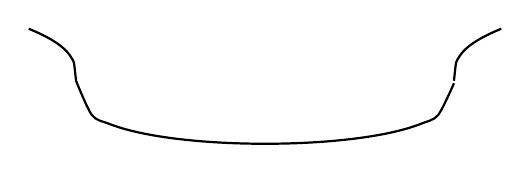
\begin{tikzpicture}[yscale=0.2,xscale=0.3]
\myaxis{x}{10}{10}{y}{6}{3}
\xcoord[xshift=2mm]{8}{8} \xcoord[xshift=-3mm]{-8}{-8} \ycoord[yshift=-2mm]{-4}{-4}
\draw[thick] plot[smooth,domain=8:10]({\x},{(\x*\x-64)^(1/3)});
\draw[thick] plot[smooth,domain=-8:-10]({\x},{(\x*\x-64)^(1/3)});
\draw[thick] plot[smooth,domain=-8:8]({\x},{-(64-\x*\x)^(1/3)});
\end{tikzpicture}
\end{center}
\vfill
}
\end{frame}
%----------------------------------------------------------------------------------------

%----------------------------------------------------------------------------------------
%----------------------------------------------------------------------------------------
\begin{frame}[t]{Let's Graph}\AnswerYes\MoreSpace\QuestionBar{2}{3}
\unote{Example~\eref{text}{eg_3_6_6}}
\[f(x)=\frac{x^2+x}{(x+1)(x^2+1)^2}\]\pause

Note: for $x \neq -1$, $f(x) = \dfrac{x(x+1)}{(x+1)(x^2+1)^2} = \dfrac{x}{(x^2+1)^2}$\pause


\[g(x):=\frac{x}{(x^2+1)^2}\]\pause

\begin{align*}
g'(x)&=\dfrac{1-3x^2}{(x^2+1)^3} \\
g''(x)&=\dfrac{12x(x^2-1)}{(x^2+1)^4}
\end{align*}
\end{frame}
%----------------------------------------------------------------------------------------
\begin{frame}<handout:0>\AnswerBar{2}{3}\unote{Example~\eref{text}{eg_3_6_6}}
\color{answercolor}
\[f(x)=\frac{x^2+x}{(x+1)(x^2+1)^2}\]\pause
When $x \neq 1$, $f(x)=g(x)$. So, $f(x)$ looks like $g(x)$ except it has a removable discontinuity (hole) at $x=1$. Let's graph 
\[g(x)=\frac{x}{(x^2+1)^2}\]
\begin{itemize}\color{answercolor}
\item Domain: all real numbers
\item HA: $y=0$ on both sides
\item VA: none
\item Intercepts: $(0,0)$
\item Odd symmetry
\item CP: $x=\pm\frac1{\sqrt 3}$; associated points: $\left(-\frac1{\sqrt 3} ,- \frac{3\sqrt3}{16} \right)$ and 
$\left(\frac1{\sqrt 3} , \frac{3\sqrt3}{16} \right)$
\end{itemize}
\end{frame}
%----------------------------------------------------------------------------------------
\begin{frame}<handout:0>\AnswerBar{2}{3}\unote{Example~\eref{text}{eg_3_6_6}}
\color{answercolor}
\begin{itemize}\color{answercolor}
\item Increasing on $\left(-\frac1{\sqrt 3}, \frac1{\sqrt 3}\right)$ and decreasing on $\left(-\infty,-\frac1{\sqrt 3}\right)\cup\left(\frac1{\sqrt 3},\infty\right)$

\begin{tikzpicture}
\myaxis{x}{2}{2}{y}{.5}{.5}
\xcoord{0.6}{}%{\frac{1}{\sqrt 3}}
\xcoord{-0.6}{}%{-\frac{1}{\sqrt 3}}
\ycoord{0.3}{}%{\frac{9\sqrt 3}{16}}
\ycoord{-0.3}{}%{-\frac{9\sqrt 3}{16}}
\draw[dashed] (-2,-.1)--(-1,-.1)--(-.6,-.3)--(.6,.3)--(1,.1)--(2,.1);
\draw (1,.125)node[opendot]{};
\end{tikzpicture}

\item  $g''$ is given (nearly) factored, so we can see its sign changes at $x=-1,0,1$. Concavity:

\begin{center}
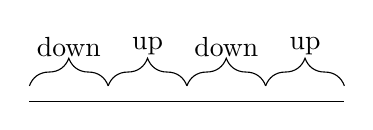
\begin{tikzpicture}
\draw (-2,0)--(2,0);
\xcoord{-1}{-1} \xcoord{0}{0} \xcoord{1}{1}
\draw[decorate, decoration={brace,amplitude=10pt}] (-2,.2)--(-1,.2)node[midway,yshift=5mm]{down};
\draw[decorate, decoration={brace,amplitude=10pt}] (-1,.2)--(0,.2)node[midway,yshift=5mm]{up};
\draw[decorate, decoration={brace,amplitude=10pt}] (-0,.2)--(1,.2)node[midway,yshift=5mm]{down};
\draw[decorate, decoration={brace,amplitude=10pt}] (1,.2)--(2,.2)node[midway,yshift=5mm]{up};
\end{tikzpicture}
\end{center}
\end{itemize}\vfill

\begin{center}
\begin{tikzpicture}[scale=2]
\myaxis{x}{2}{2}{y}{.5}{.5}
\xcoord{0.6}{\frac{1}{\sqrt 3}}
\xcoord{-0.6}{-\frac{1}{\sqrt 3}}
\ycoord{0.3}{\frac{9\sqrt 3}{16}}
%\ycoord{-0.3}{-\frac{9\sqrt 3}{16}}
\ycoord{-0.3}{}
\xcoord{1}{1} \xcoord{-1}{-1}
\draw[thick] plot[smooth,domain=-2:2](\x,{\x/(\x*\x+1)^2});
\draw (1,.25)node[opendot]{};
\end{tikzpicture}
\end{center}

\end{frame}
%----------------------------------------------------------------------------------------
%----------------------------------------------------------------------------------------
%----------------------------------------------------------------------------------------

%%----------------------------------------------------------------------------------------
\begin{frame}[t]{Let's Graph}
\AnswerYes\QuestionBar{3}{3}
\unote{Example~\eref{text}{APPsketchC}}
\[f(x)=x(x-1)^{2/3}\]
\vfill
\begin{itemize}
\item[\textbullet] $f'(x)=\dfrac{5x-3}{3\sqrt[3]{x-1}}$
\item[\textbullet] $f''(x)=\dfrac{2(5x-6)}{9(\sqrt[3]{x-1})^4}$
\pause\vfill
\item $f(3/5)\approx 0.3$
\item $f(6/5)\approx 0.4$
\end{itemize}
\end{frame}
%----------------------------------------------------------------------------------------
\begin{frame}<handout:0>
\AnswerBar{3}{3}\color{answercolor}
\unote{Example~\eref{text}{APPsketchC}}
\begin{itemize}\color{answercolor}
\item Domain: all reals
\item VA: none
\item HA: none
\item Intercepts: $(0,0)$, $(1,0)$
\item Symmetry: not even, not odd, not periodic
\item CP: $x=\frac35$ ($y\approx 0.3$); SP $x=1$ ($y=0$).\\ 
   Near the SP, first deriv is very large, so function looks vertical.
\begin{tikzpicture}[xscale=2]
\myaxis{x}{1}{2}{y}{1}{1}
\draw[thick] (.5,.3)--(.7,.3)node[midway,vertex]{};
\xcoord{3/5}{\frac35}
\draw (1,0)node[vertex,label=below:1]{};
\draw[thick] (1,.2)--(1,-.2);
\draw (0,0)node[vertex]{};
\end{tikzpicture}
\end{itemize}
\end{frame}
%----------------------------------------------------------------------------------------
%----------------------------------------------------------------------------------------

%----------------------------------------------------------------------------------------
\begin{frame}<handout:0>
\unote{Example~\eref{text}{APPsketchC}}
\AnswerBar{3}{3}\color{answercolor}
\begin{itemize}\color{answercolor}
\item First derivative changes sign at $x=\frac35$ and $x=1$. Function is increasing on $\left(-\infty,\frac35\right)\cup(1,\infty)$ and decreasing on $\left(\frac35,1\right)$.

\begin{center}
\begin{tikzpicture}[xscale=2]
\myaxis{x}{1}{2}{y}{1}{1}
\draw[thick] (.5,.3)--(.7,.3)node[midway,vertex]{};
\xcoord{3/5}{\frac35}
\draw (1,0)node[vertex,label=below:1]{};
\draw[thick] (1,.2)--(1,-.2);
\draw (0,0)node[vertex]{};
\draw[thick,dashed] (-1,-1)--(0,0) sin (.6,.3) cos (1,0) -- (2,1);
\end{tikzpicture}
\end{center}

\item Second derivative changes sign at $x=\frac56$.  (Note the denominator has an even power). Function is concave down on $\left(-\infty,\frac56\right)$ and concave up on $\left(\frac56,\infty\right)$.

\begin{center}
\begin{tikzpicture}[xscale=2]
\myaxis{x}{1}{2}{y}{1}{1}
\draw[thick,C1] plot[samples=100,domain=-1:1.5](\x,{\x*((\x-1)*(\x-1))^(1/3)});
\draw[thick] (.5,.3)--(.7,.3)node[midway,vertex]{};
\xcoord{3/5}{\frac35}
\draw (1,0)node[vertex,label=below:1]{};
\draw[thick] (1,.2)--(1,-.2);
\draw (0,0)node[vertex]{};
\end{tikzpicture}
\end{center}
\end{itemize}
\end{frame}
%---------------------------------
%----------------------------------------------------------------------------------------
\begin{frame}
Ch 3.6 Review: matching
\note{Matching (as opposed to sketching) is a nice way to review specific ideas, like when a function changes signs.}
\end{frame}
%%---------------------------------
%----------------------------------------------------------------------------------------
\begin{frame}[t]{Match the Function to its Graph}\AnswerNo\QuestionBar{2}{4}
A. $f(x)=x^3(x+2)(x-2)=x^5-4x^3$\\
B. $f(x)=x(x+2)^3(x-2)=x^5+4x^4-16x^2-16x$\\
C. $f(x)=x(x+2)(x-2)^3=x^5-4x^4+16x^2-16x$\\\vfill
\begin{multicols}{2}\centering
\includegraphics[height=0.3\textheight]{C1}\\
\textcolor{C3}{I}\vfill

\includegraphics[height=0.3\textheight]{C3}\\
II\columnbreak

\includegraphics[height=0.3\textheight]{C2}
\textcolor{M5}{III}

\end{multicols}
\index{\includegraphics[height=5mm]{fig/C1}, \includegraphics[height=5mm]{fig/C2}, \includegraphics[height=5mm]{fig/C3} screenshots of graphs generated using Desmos Graphing Calculator \url{https://www.desmos.com/calculator} (accessed 13 November 2015)}

\end{frame}
%----------------------------------------------------------------------------------------

\begin{frame}\AnswerNo\QuestionBar{2}{4}
\begin{multicols}{2}\centering
\begin{enumerate}[A.]
\item $f(x)=\dfrac{x-1}{(x+1)(x+2)}$
\item $f(x)=\dfrac{(x-1)^2}{(x+1)(x+2)}$
\item $f(x)=\dfrac{x-1}{(x+1)^2(x+2)}$
\item $f(x)=\dfrac{(x-1)^2}{(x+1)^2(x+2)}$
\end{enumerate}
\end{multicols}

\COPY{0.25}{\h}
\begin{multicols}{2}\centering
\textcolor{C1}{I. }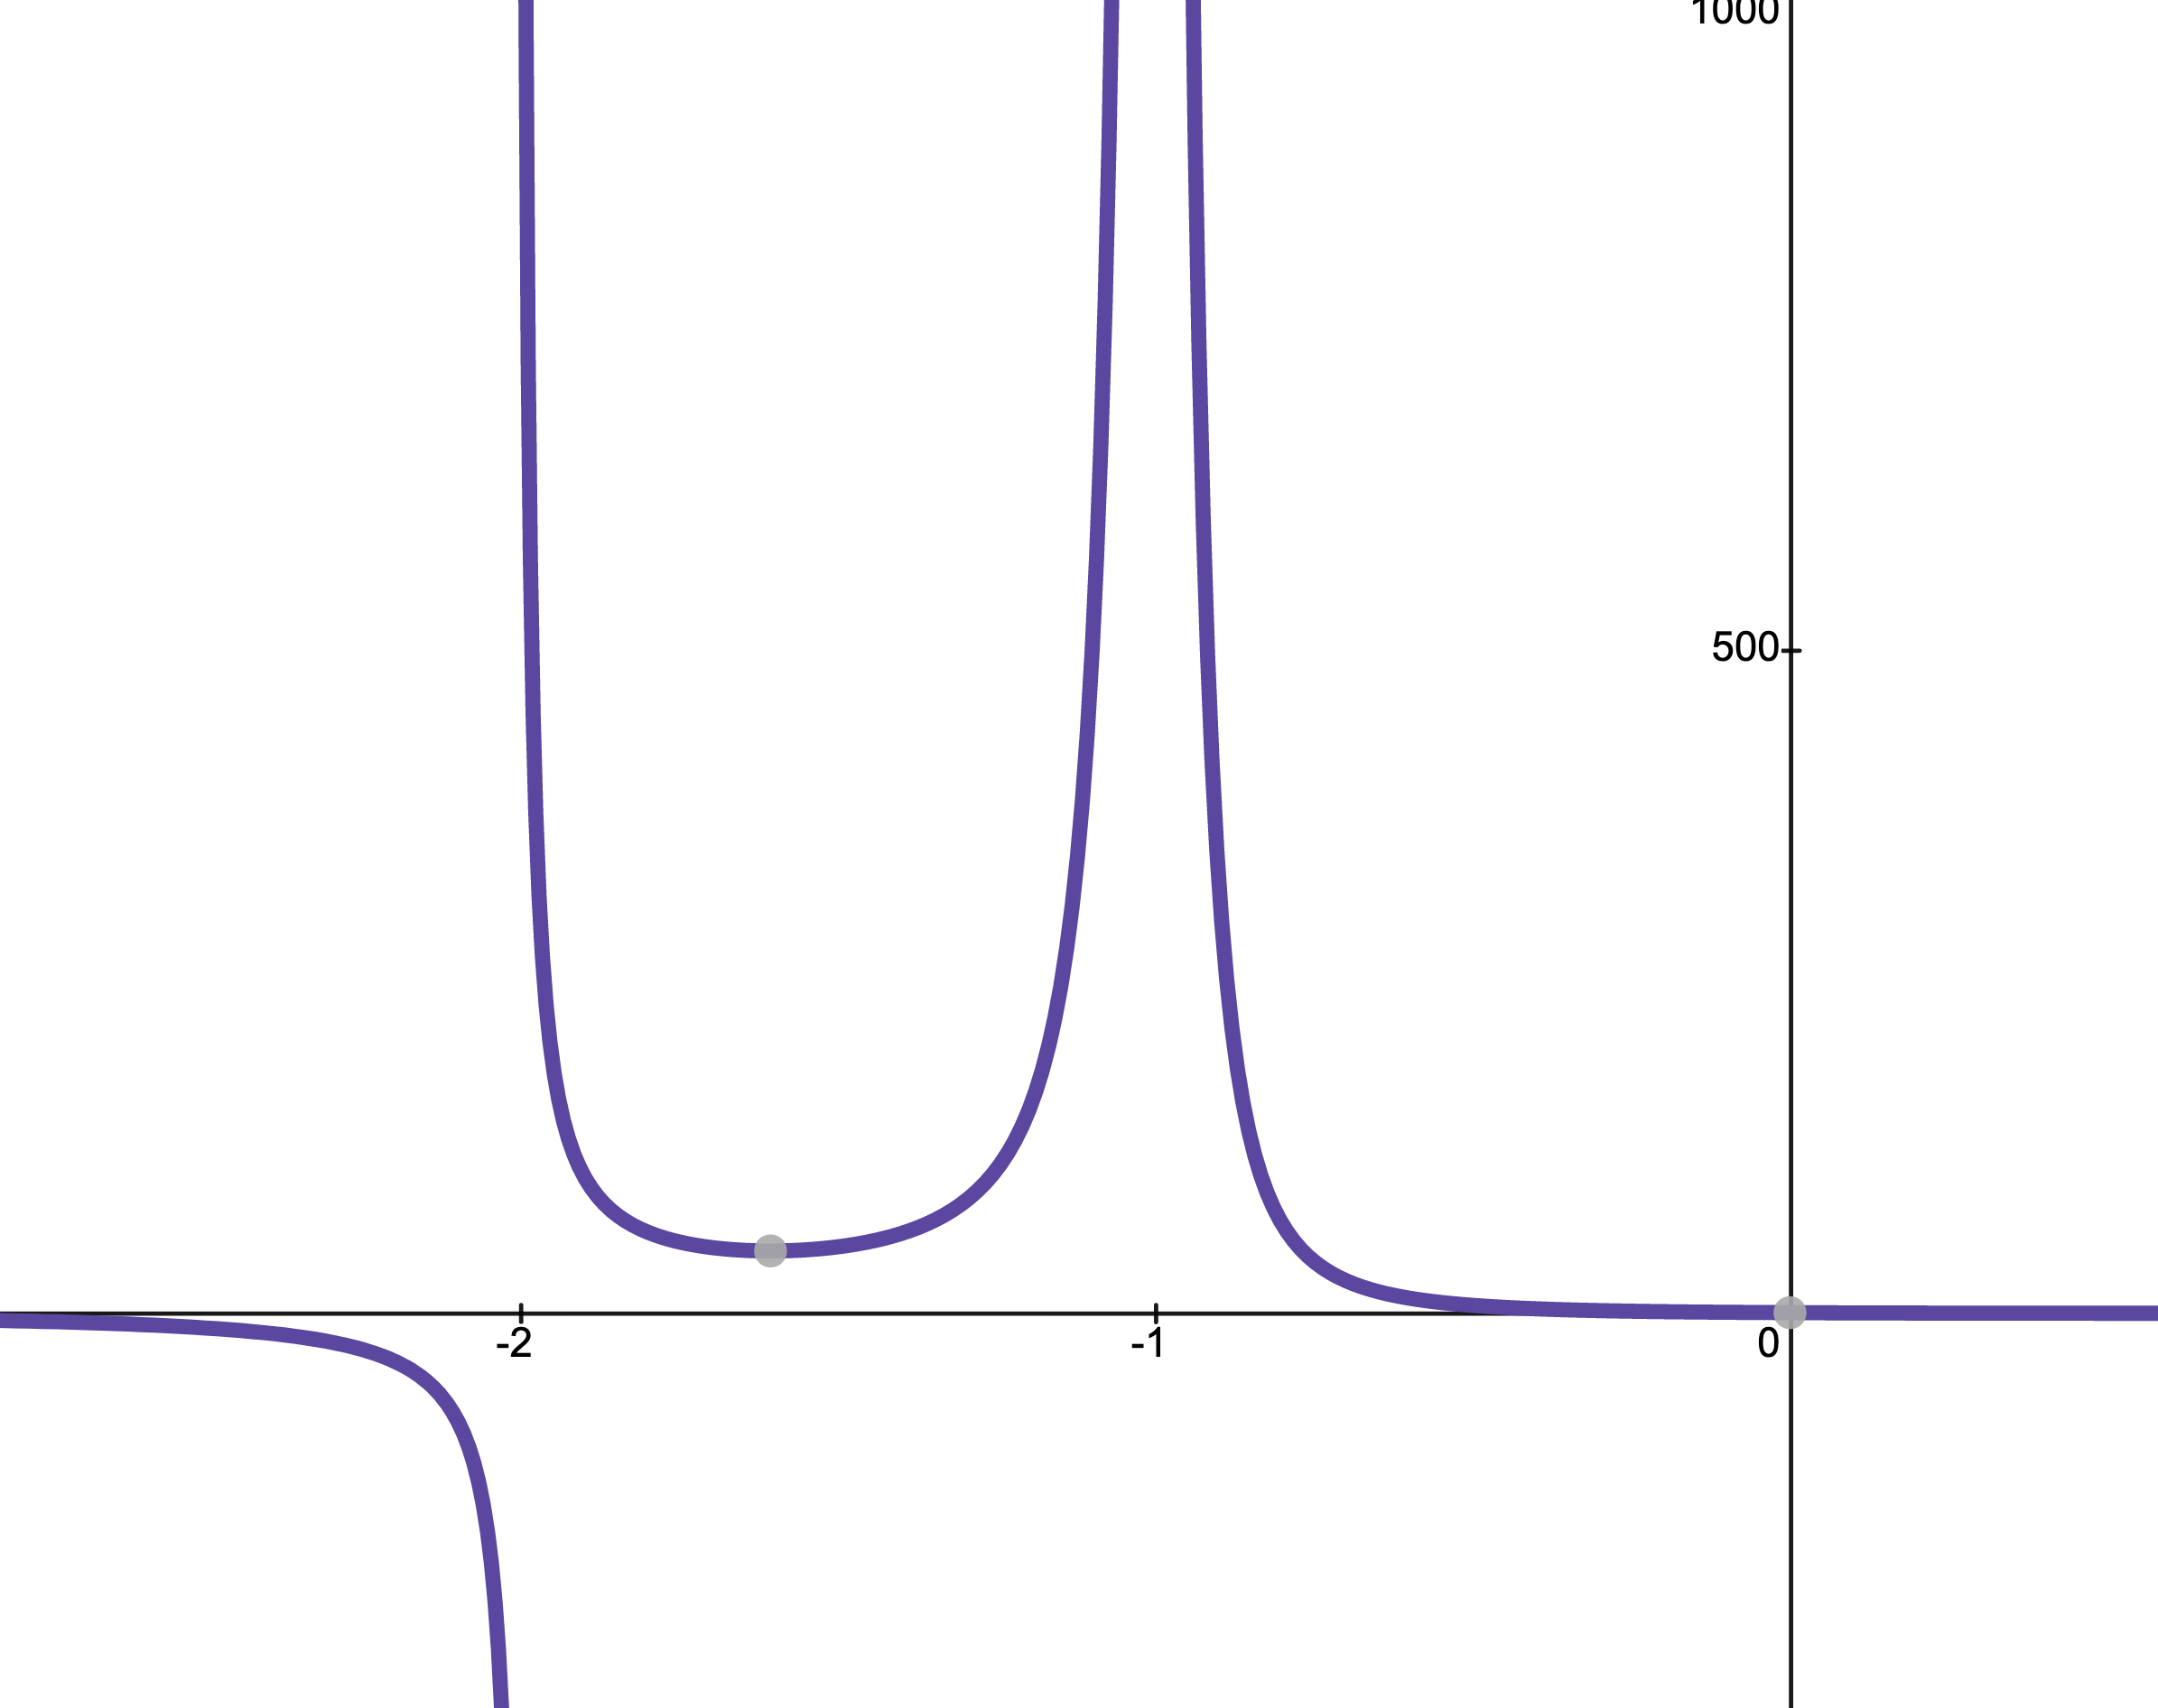
\includegraphics[height=\h\textheight]{fig/R4}\\[2em]

\textcolor{W1}{II. }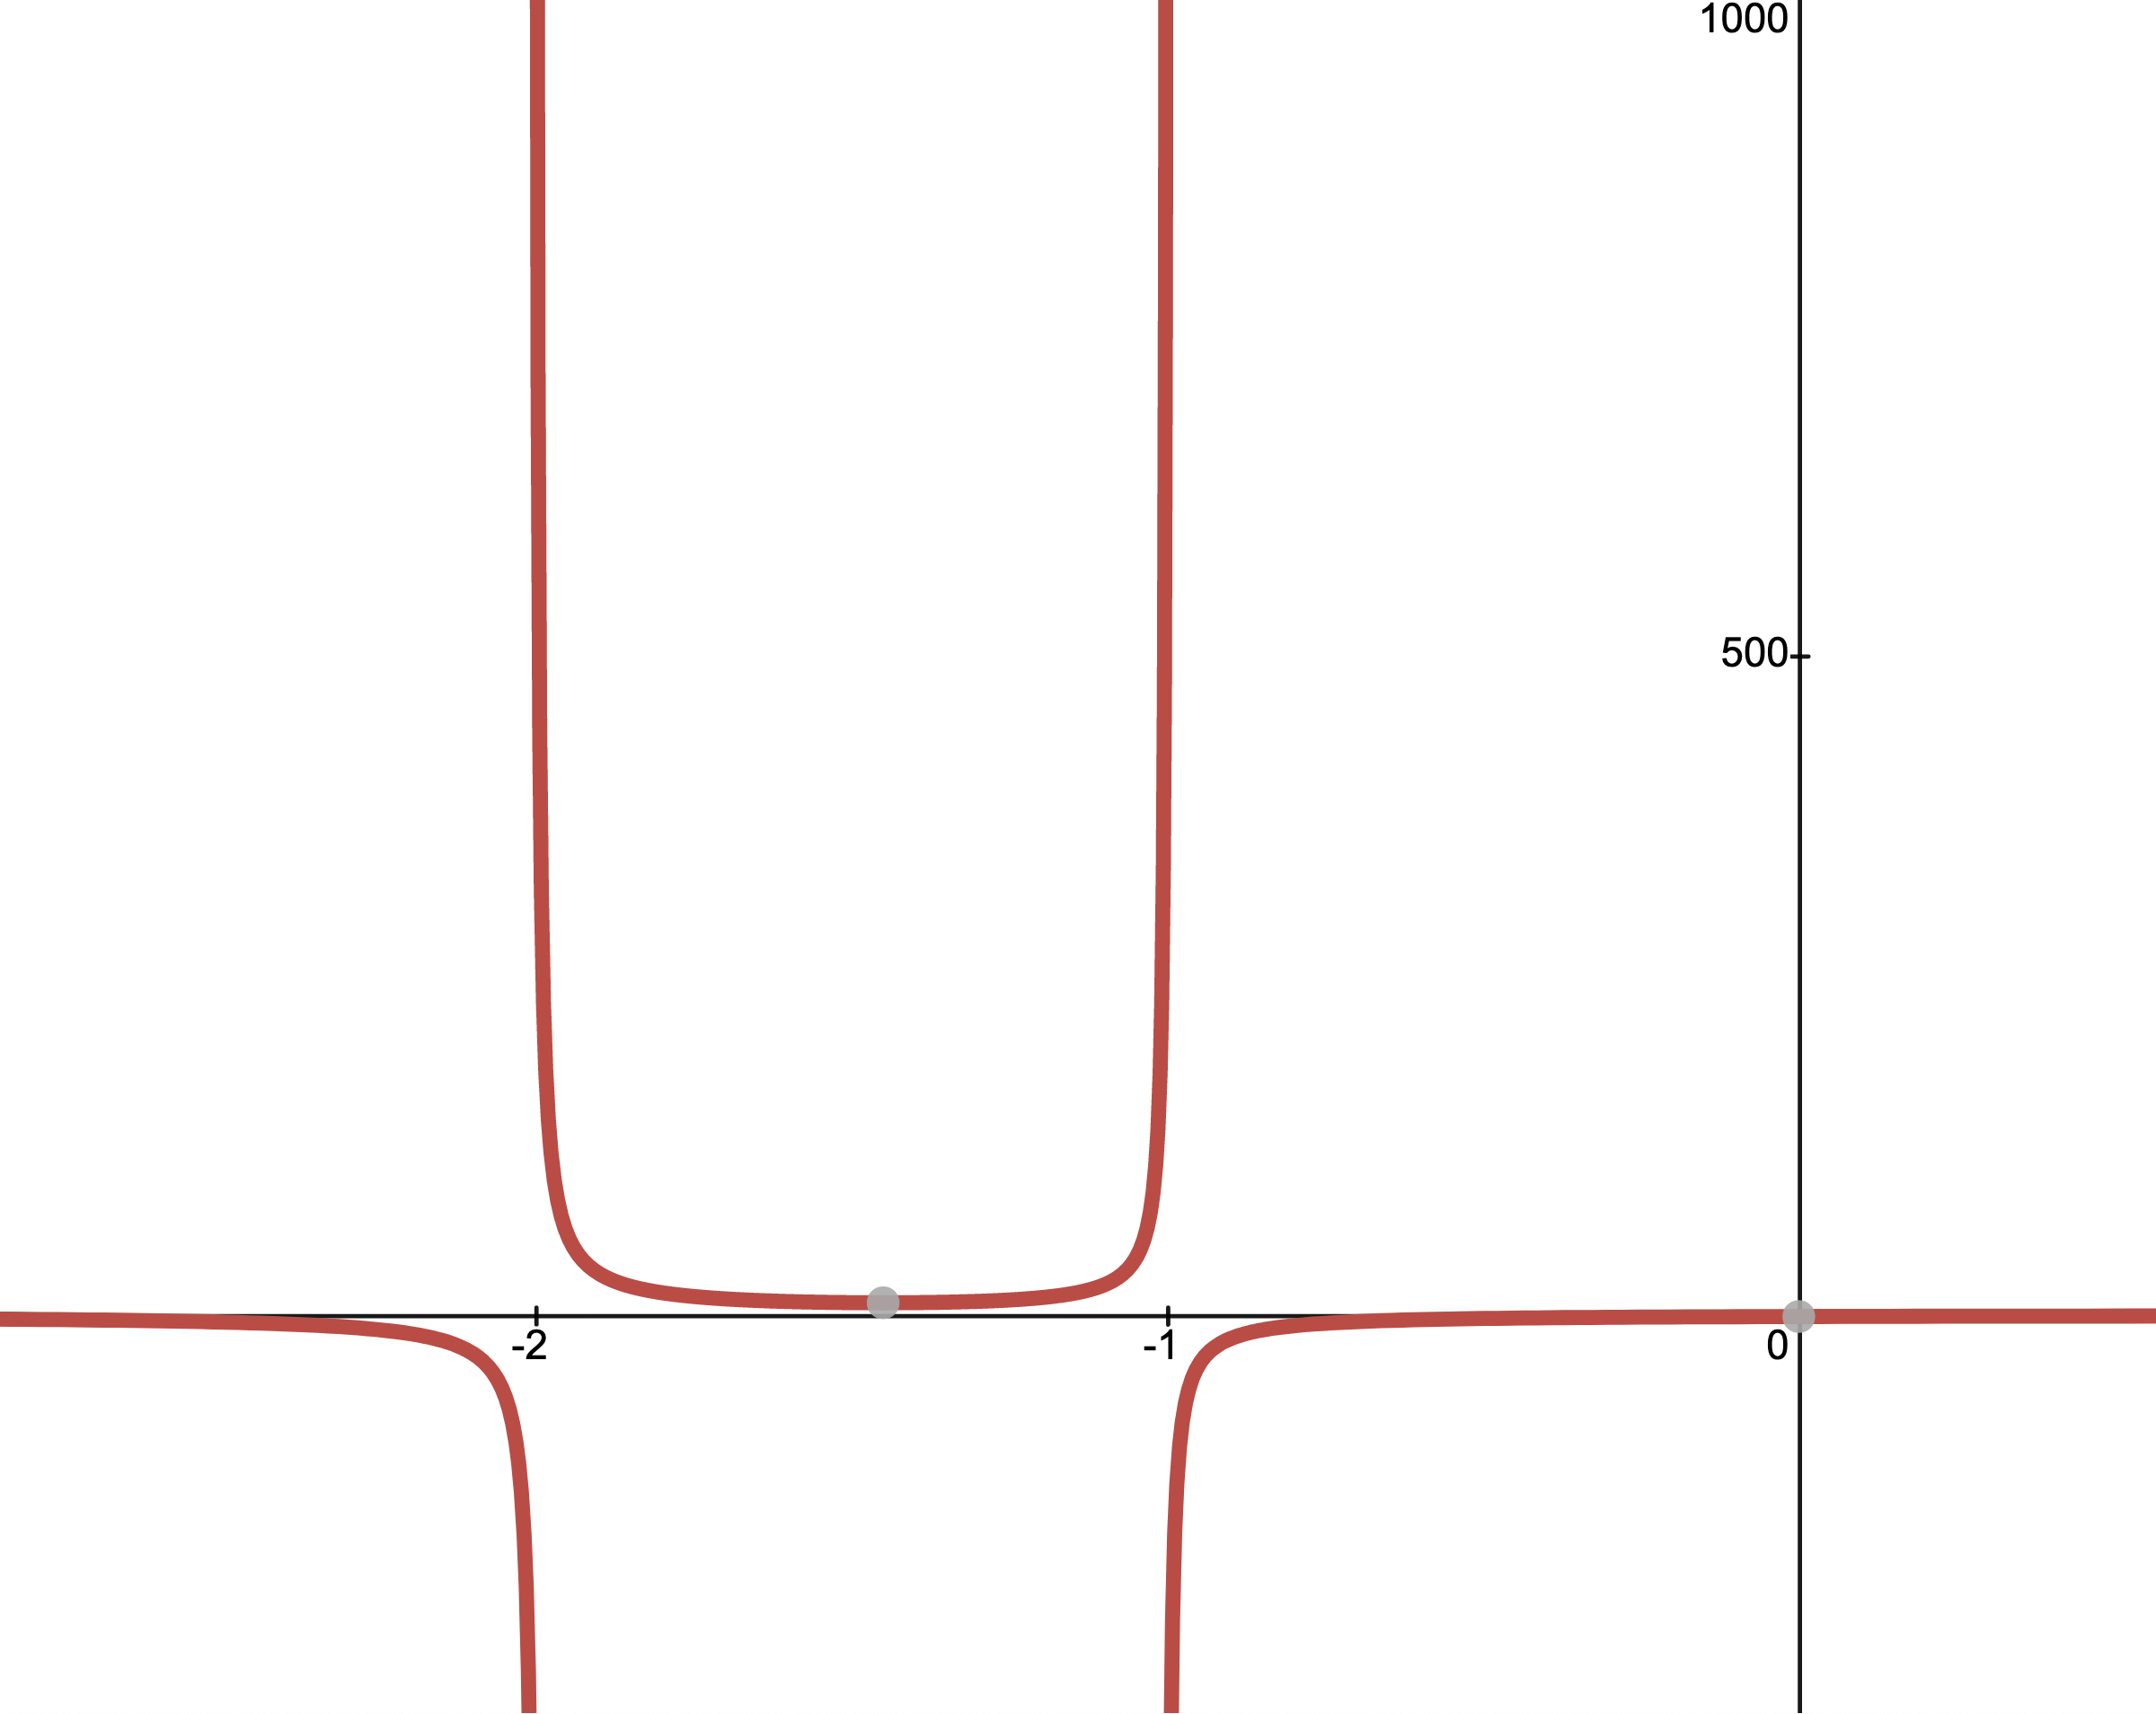
\includegraphics[height=\h\textheight]{fig/R1}\\[2em]

\textcolor{C4}{III. }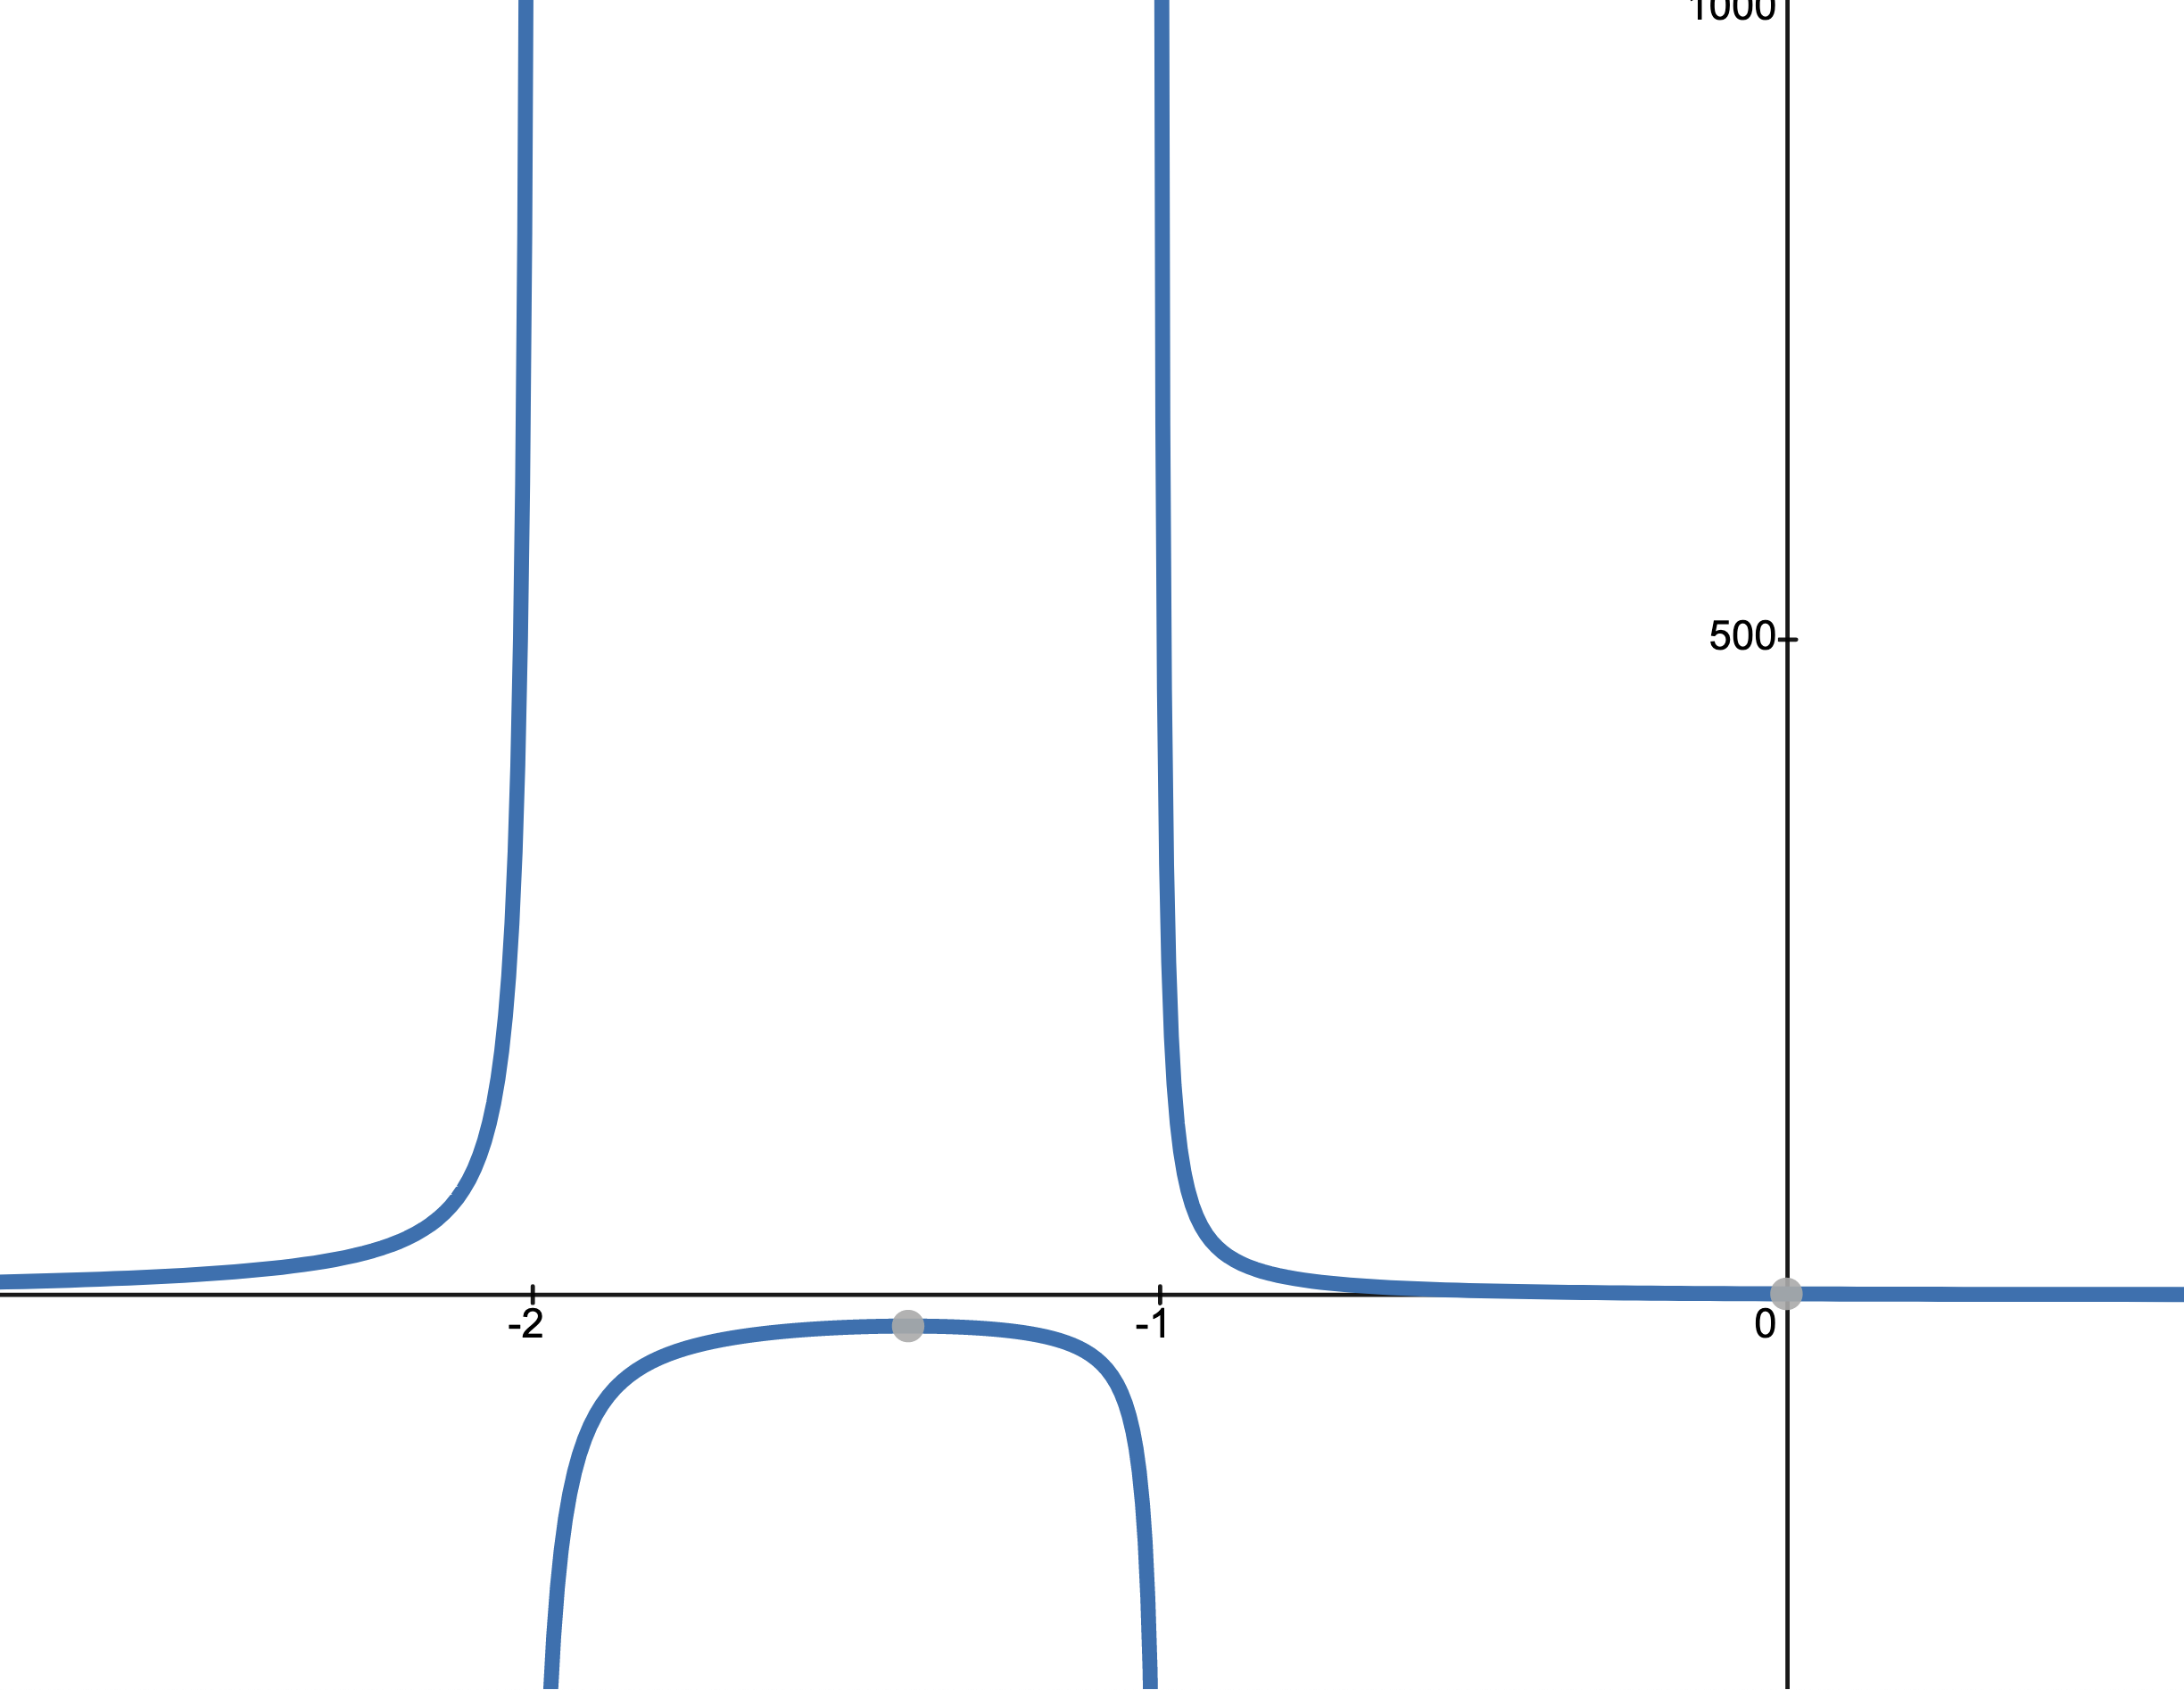
\includegraphics[height=\h\textheight]{fig/R2}\\[2em]

\textcolor{M3}{IV. }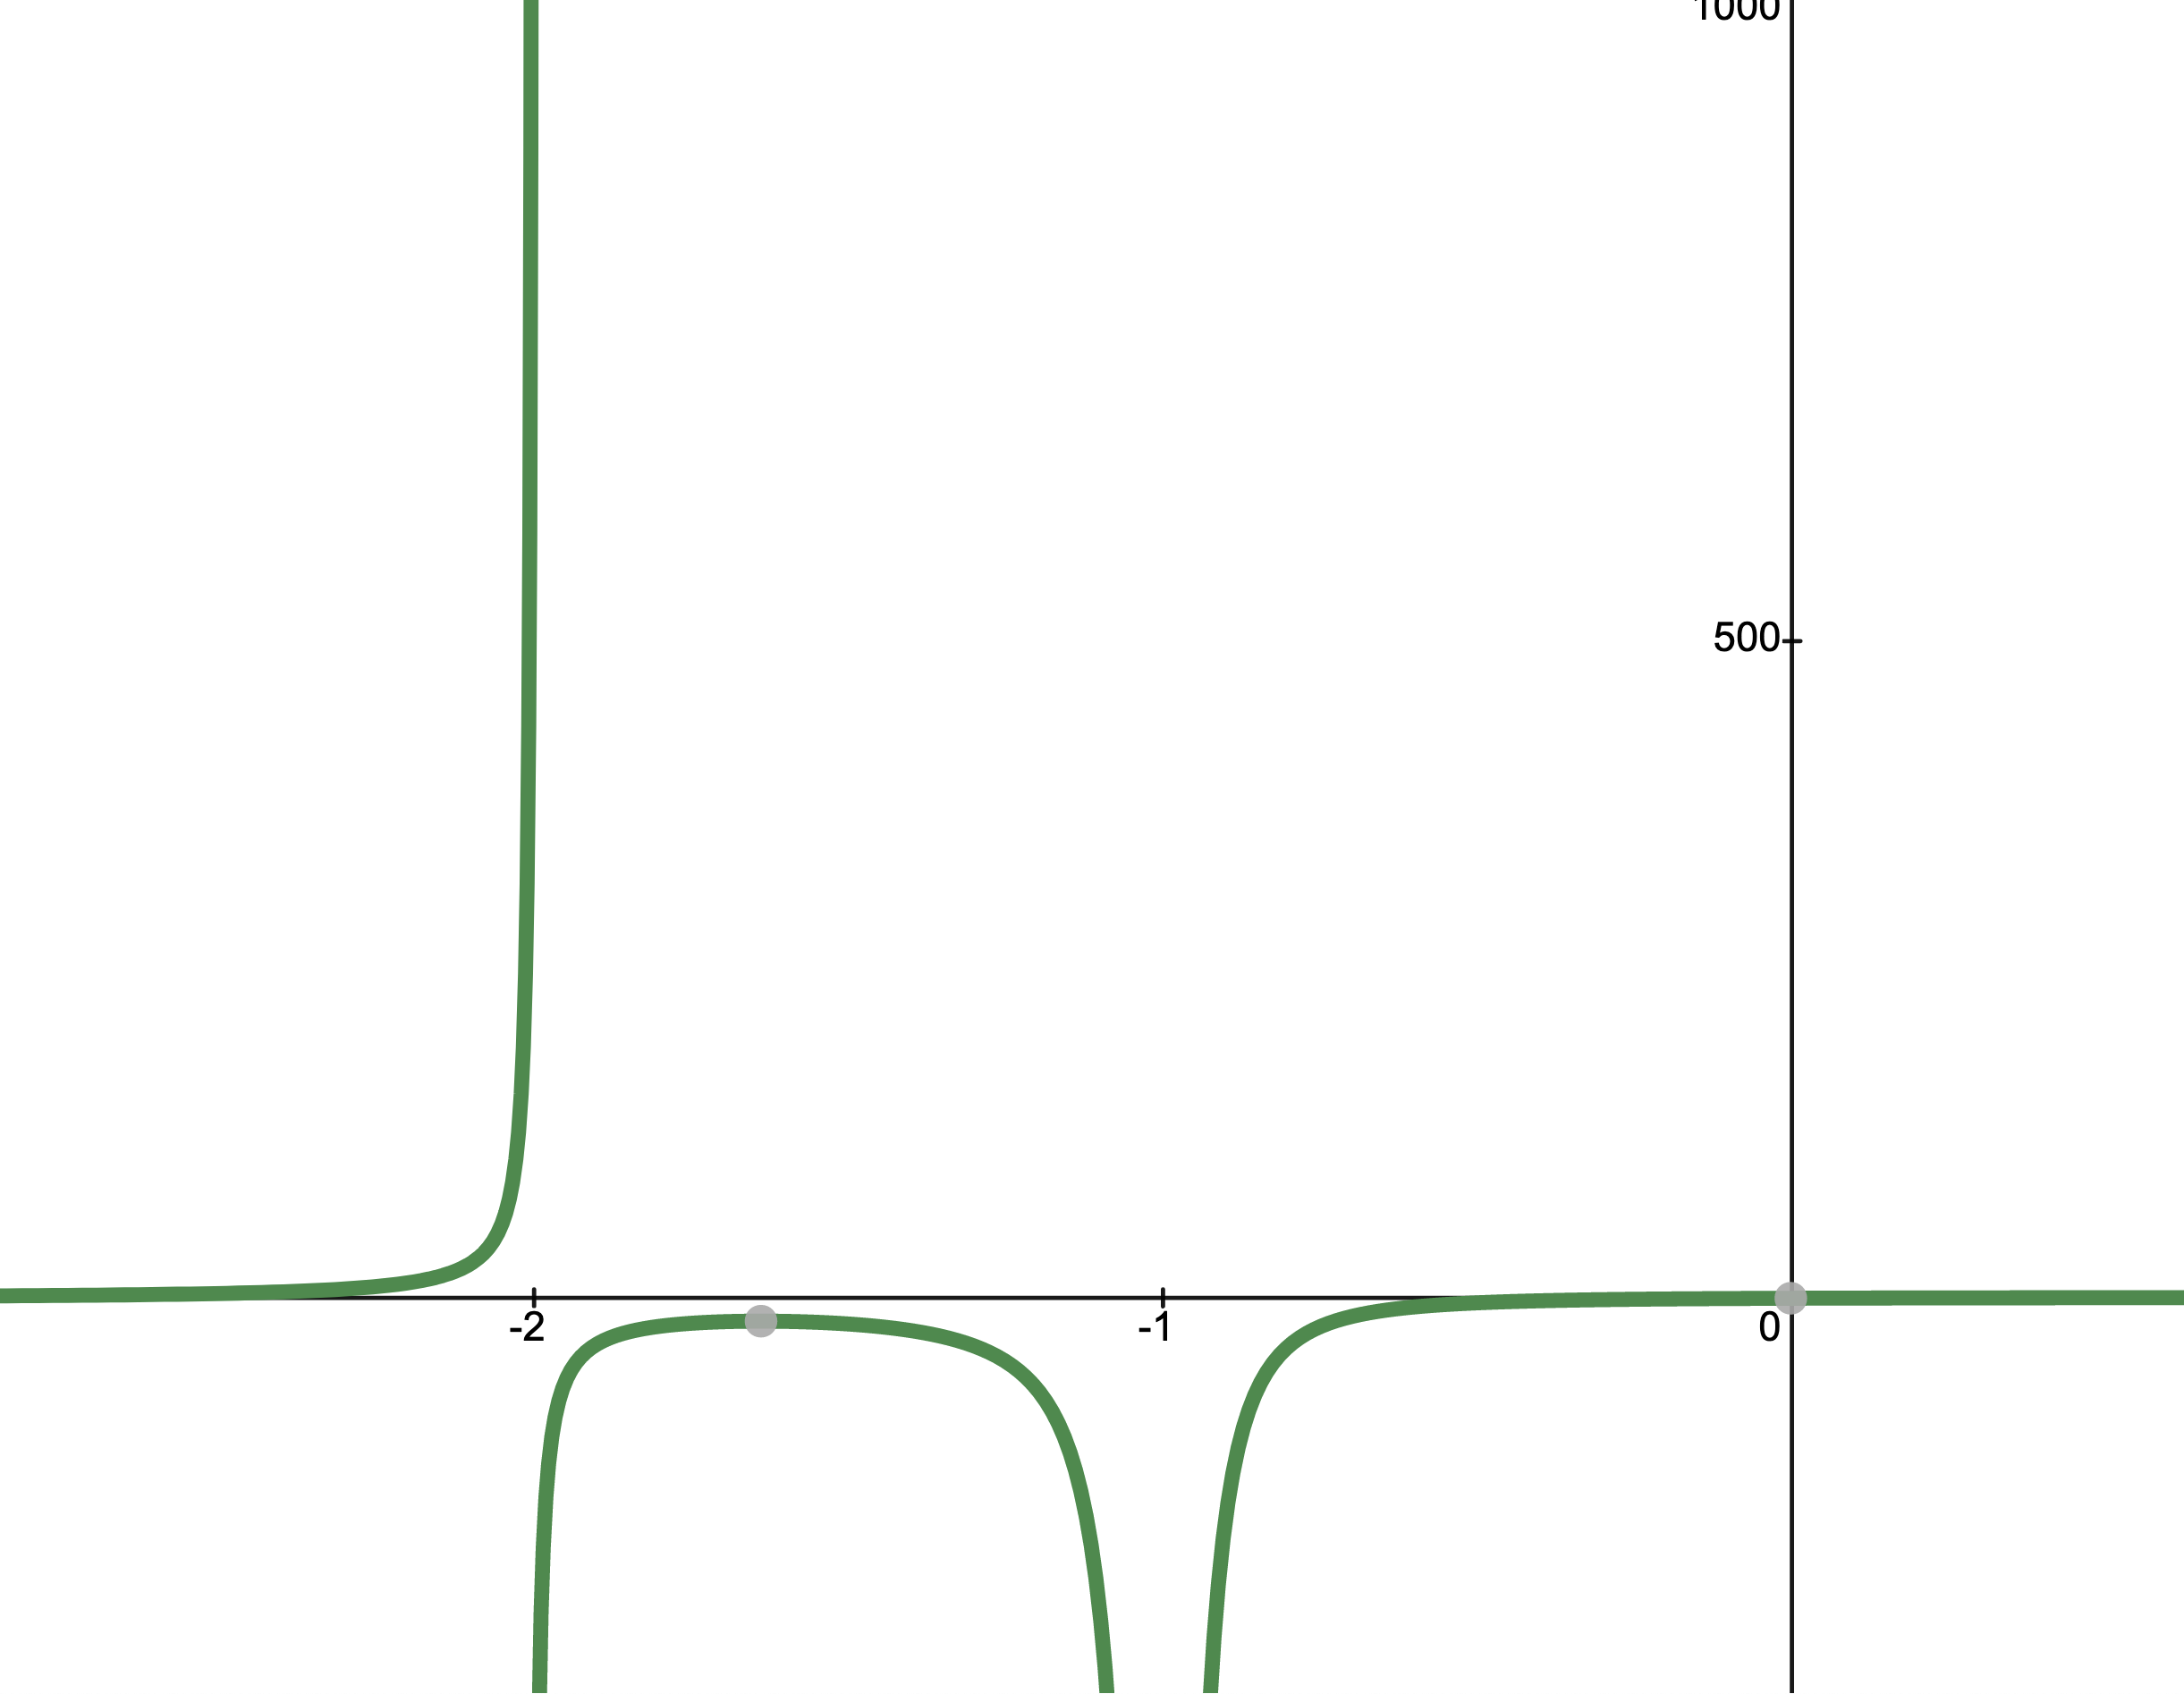
\includegraphics[height=\h\textheight]{fig/R3}\\

\end{multicols}



\index{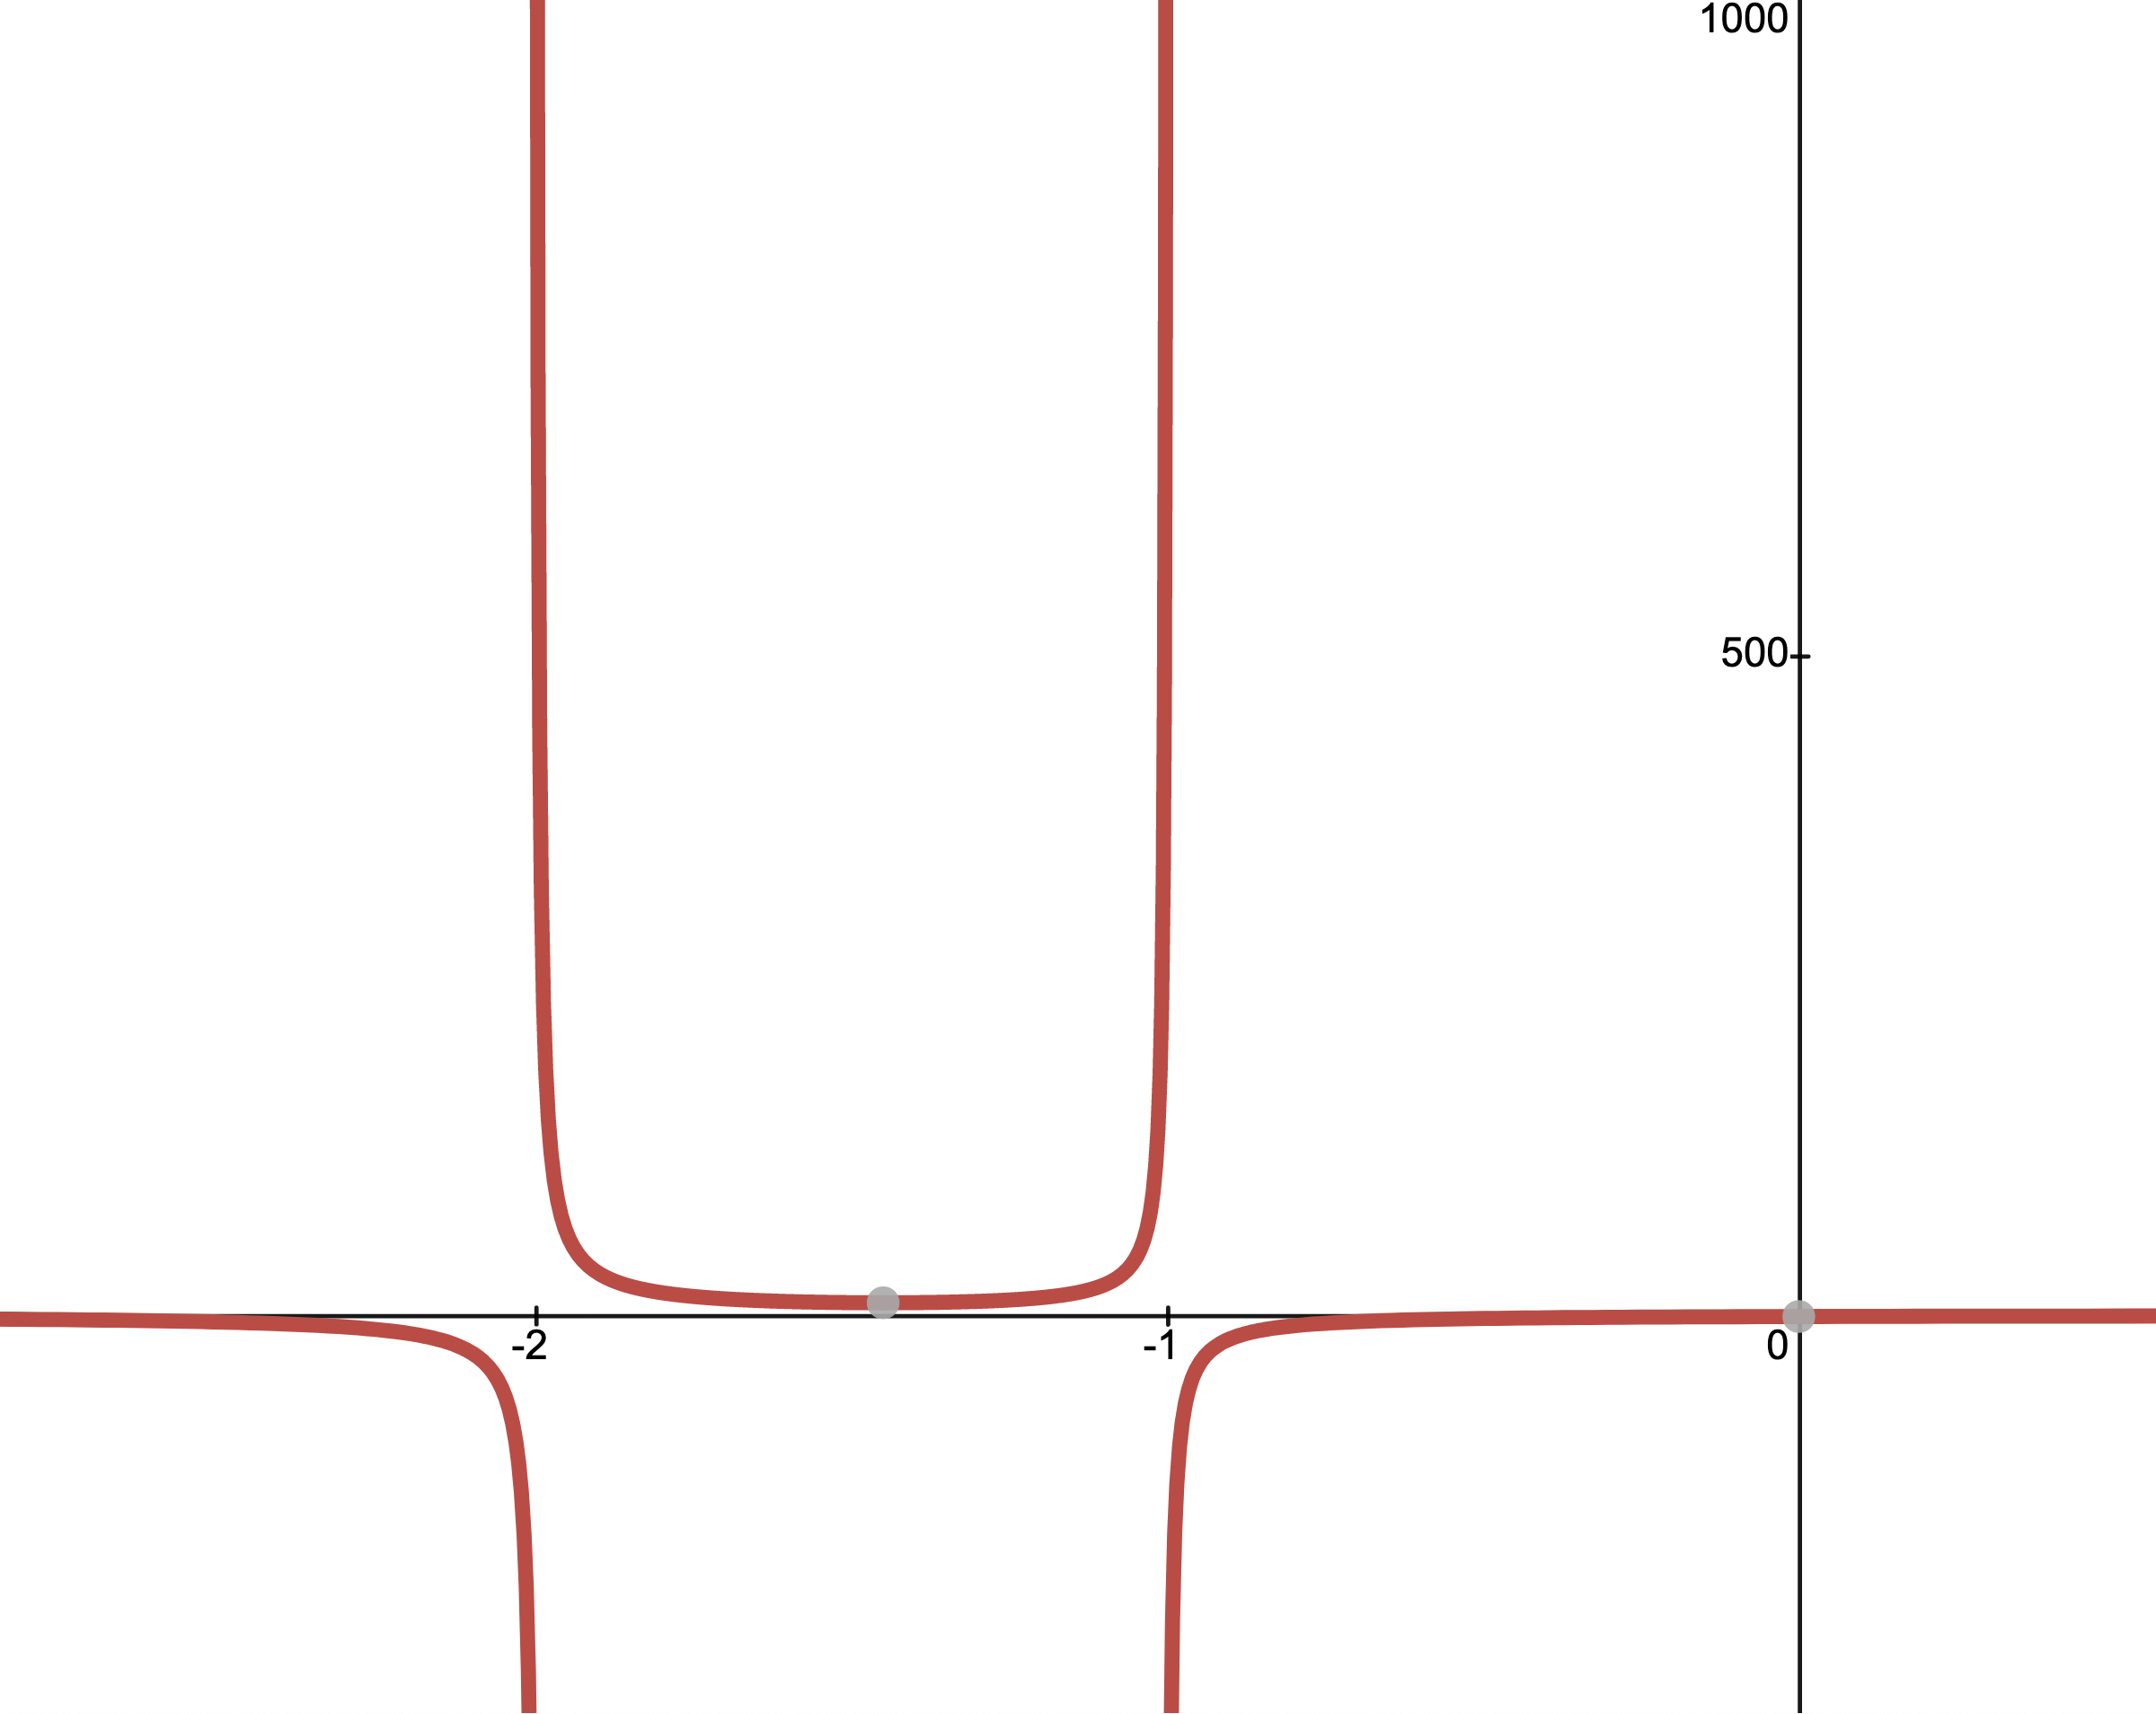
\includegraphics[height=5mm]{fig/R1}, 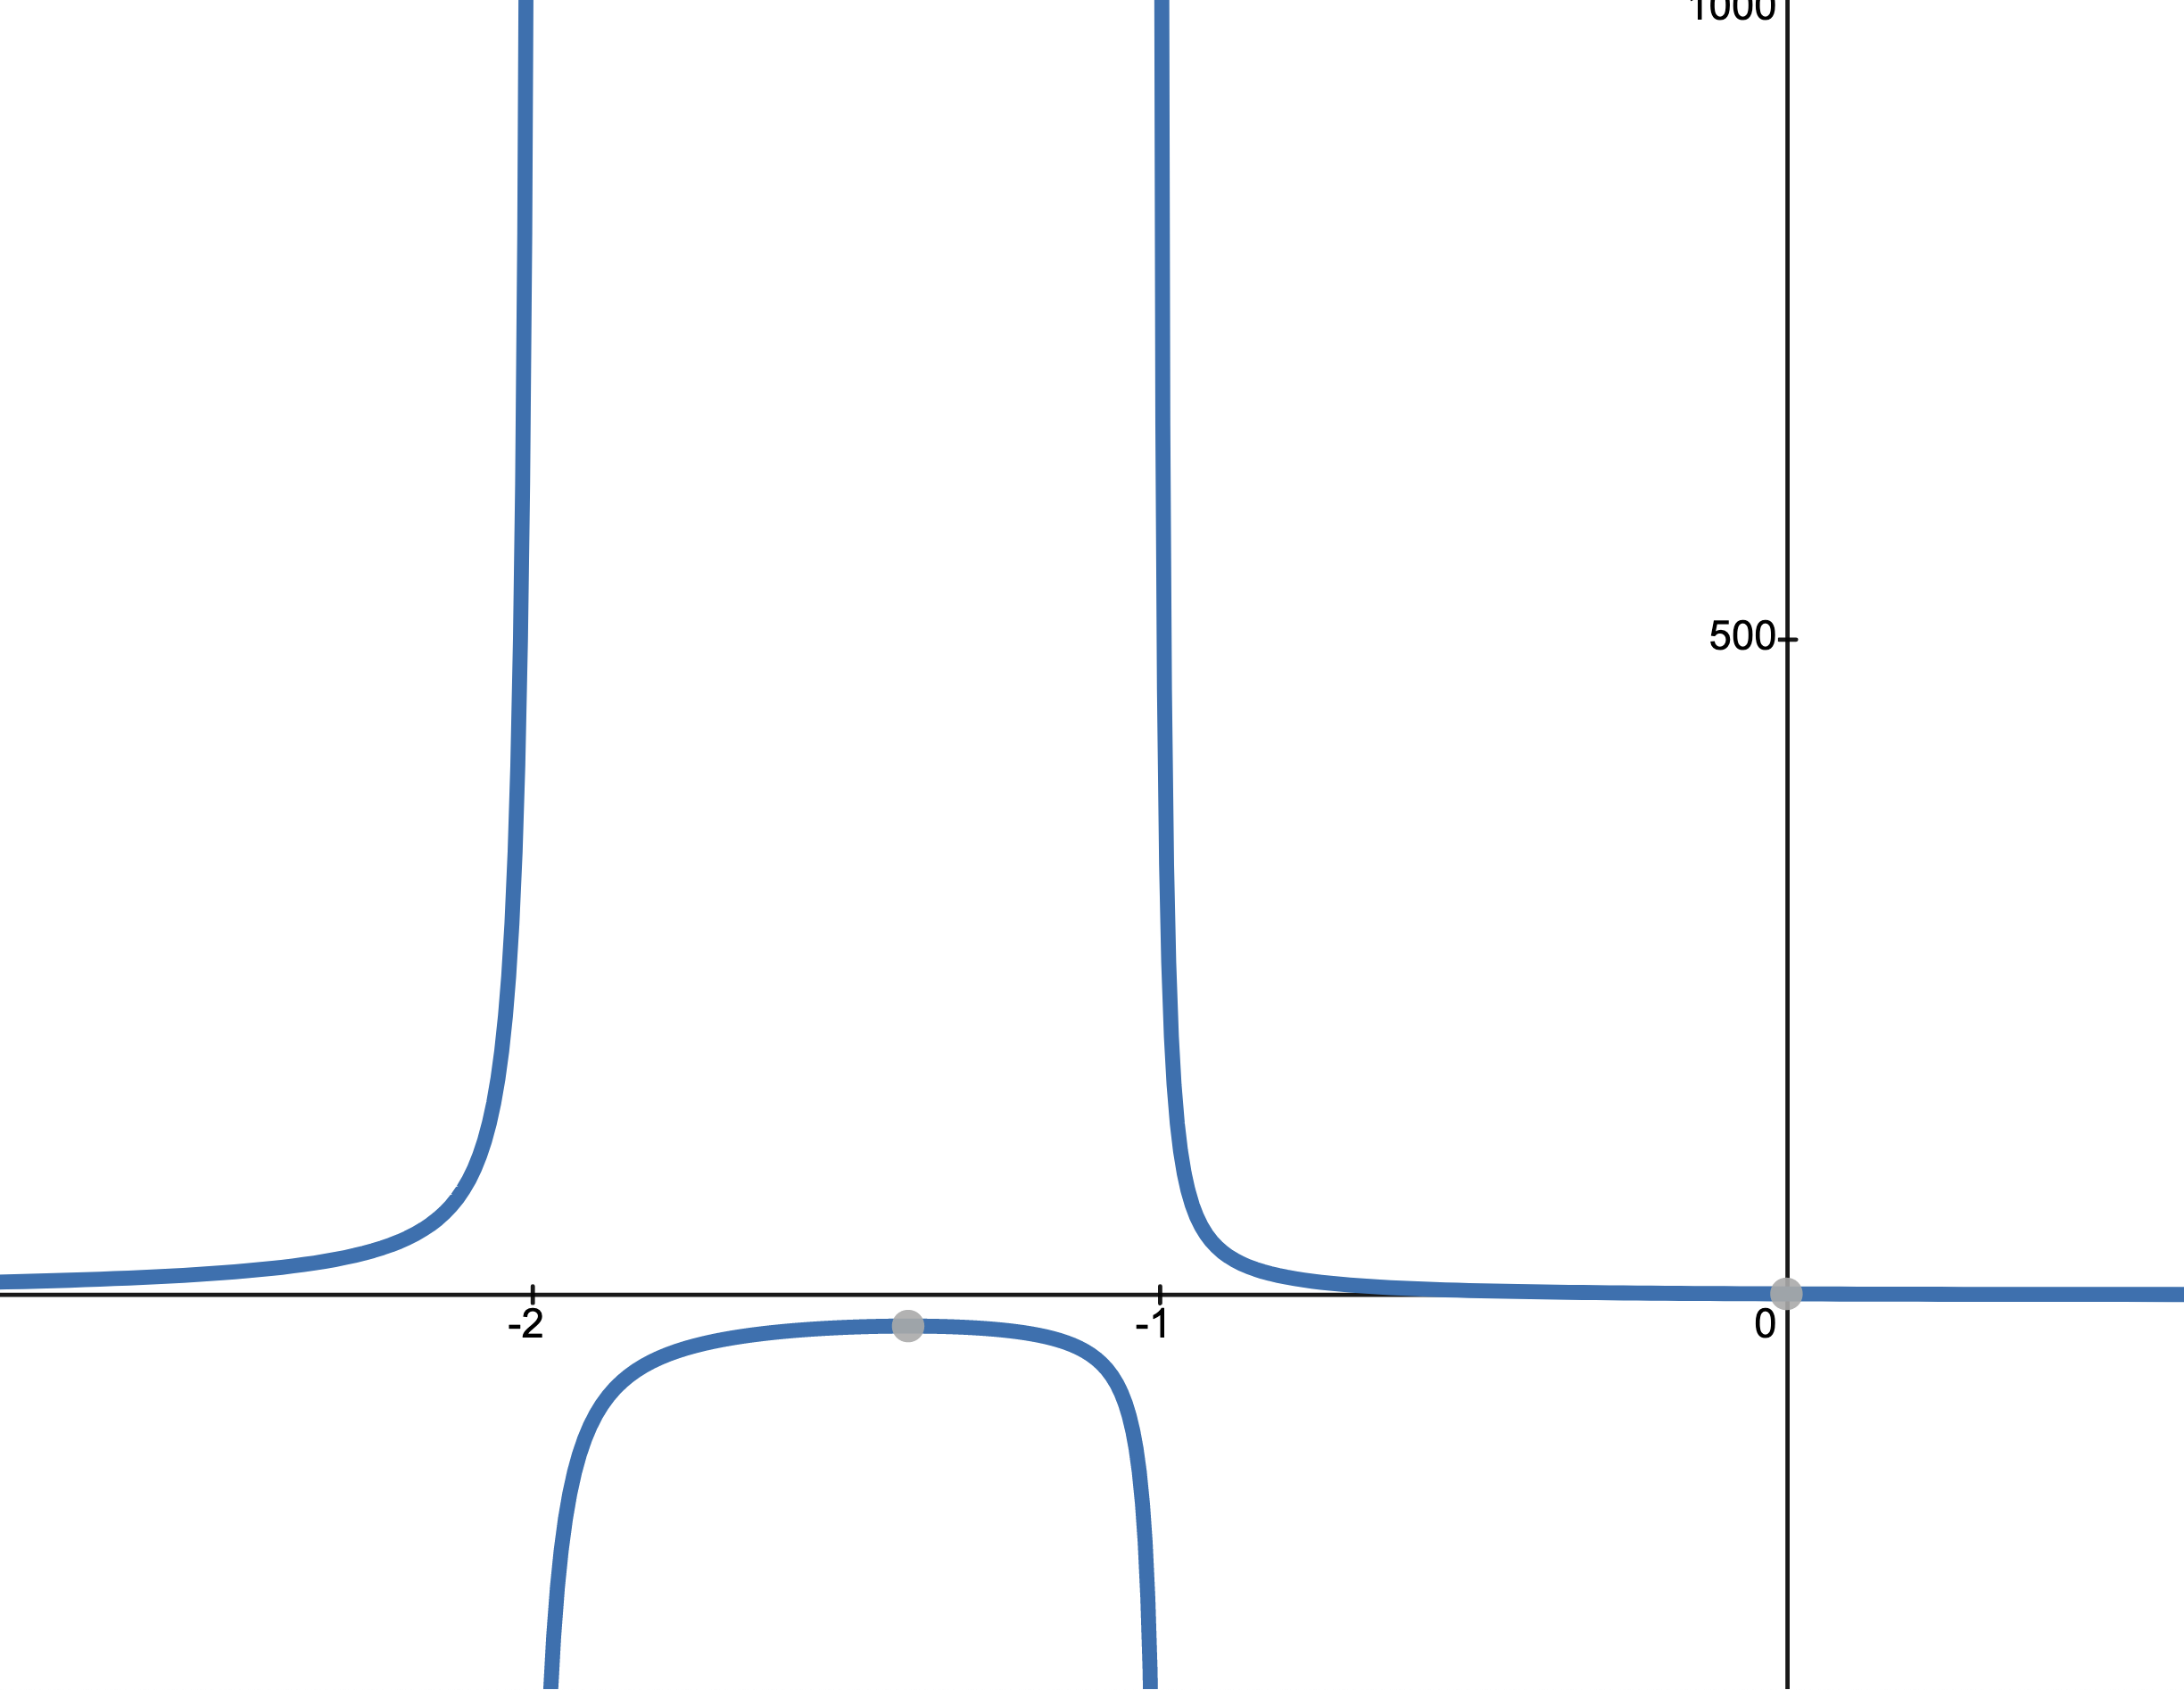
\includegraphics[height=5mm]{fig/R2}, 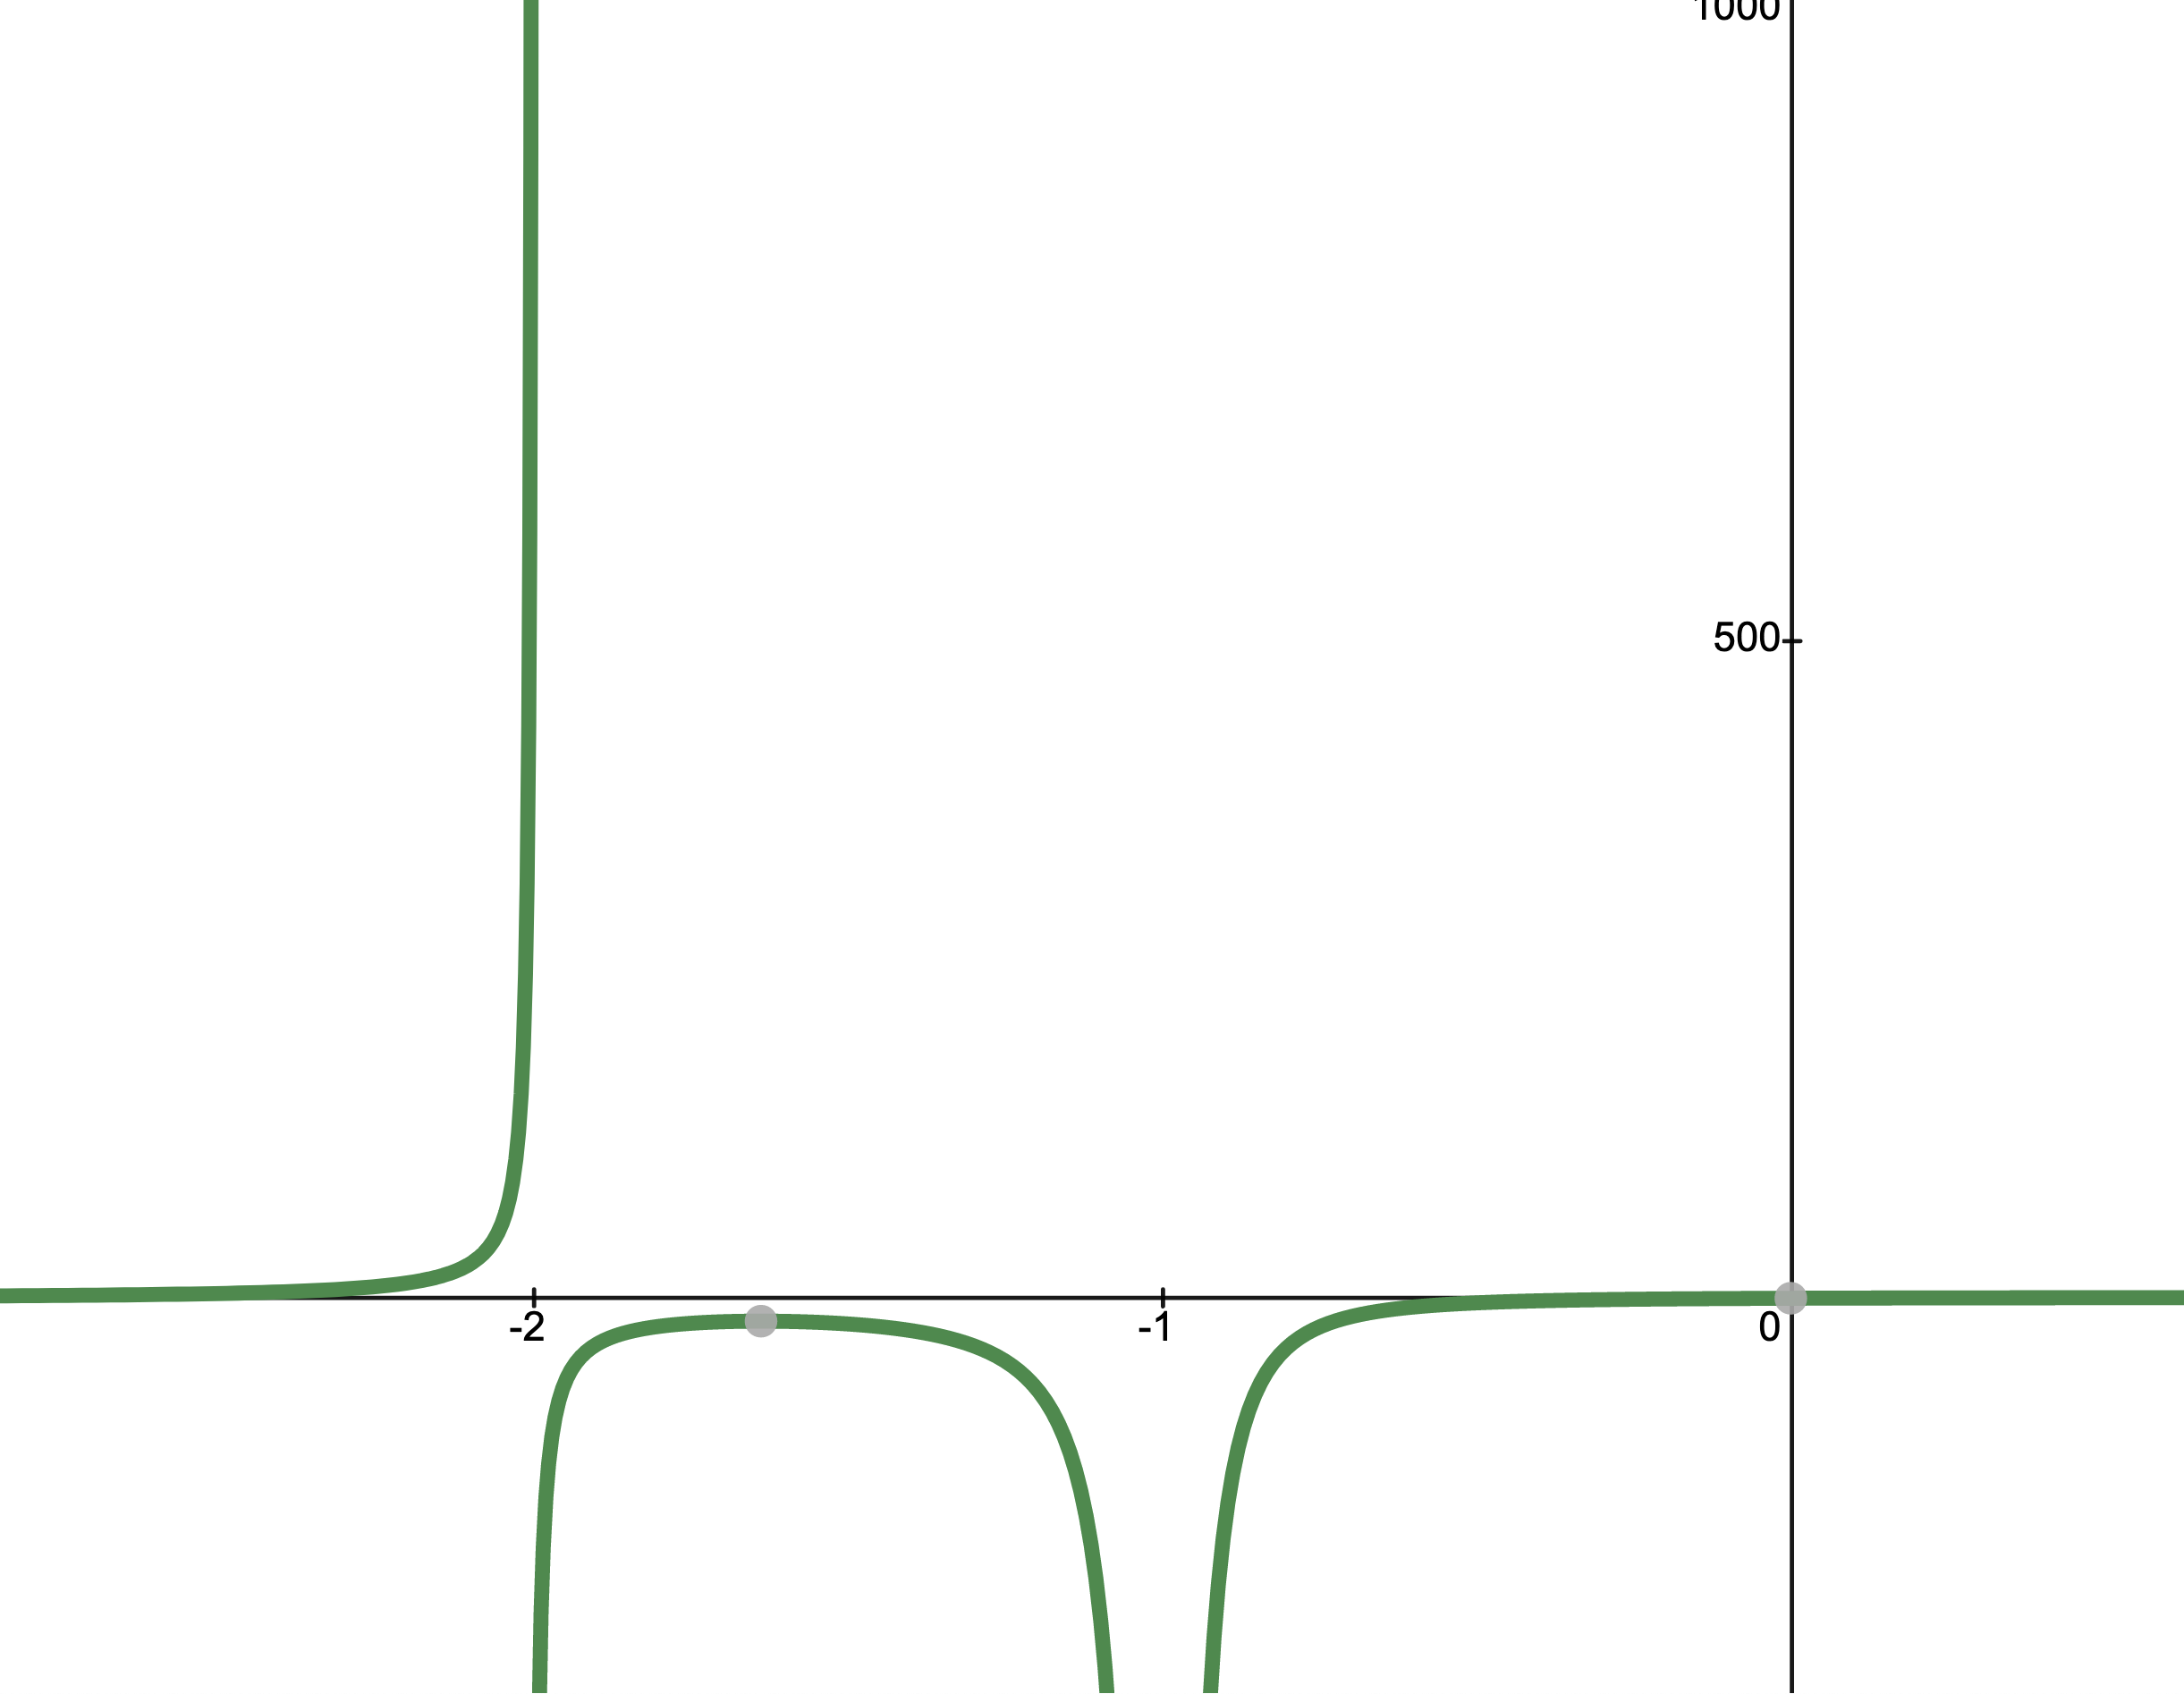
\includegraphics[height=5mm]{fig/R3}, 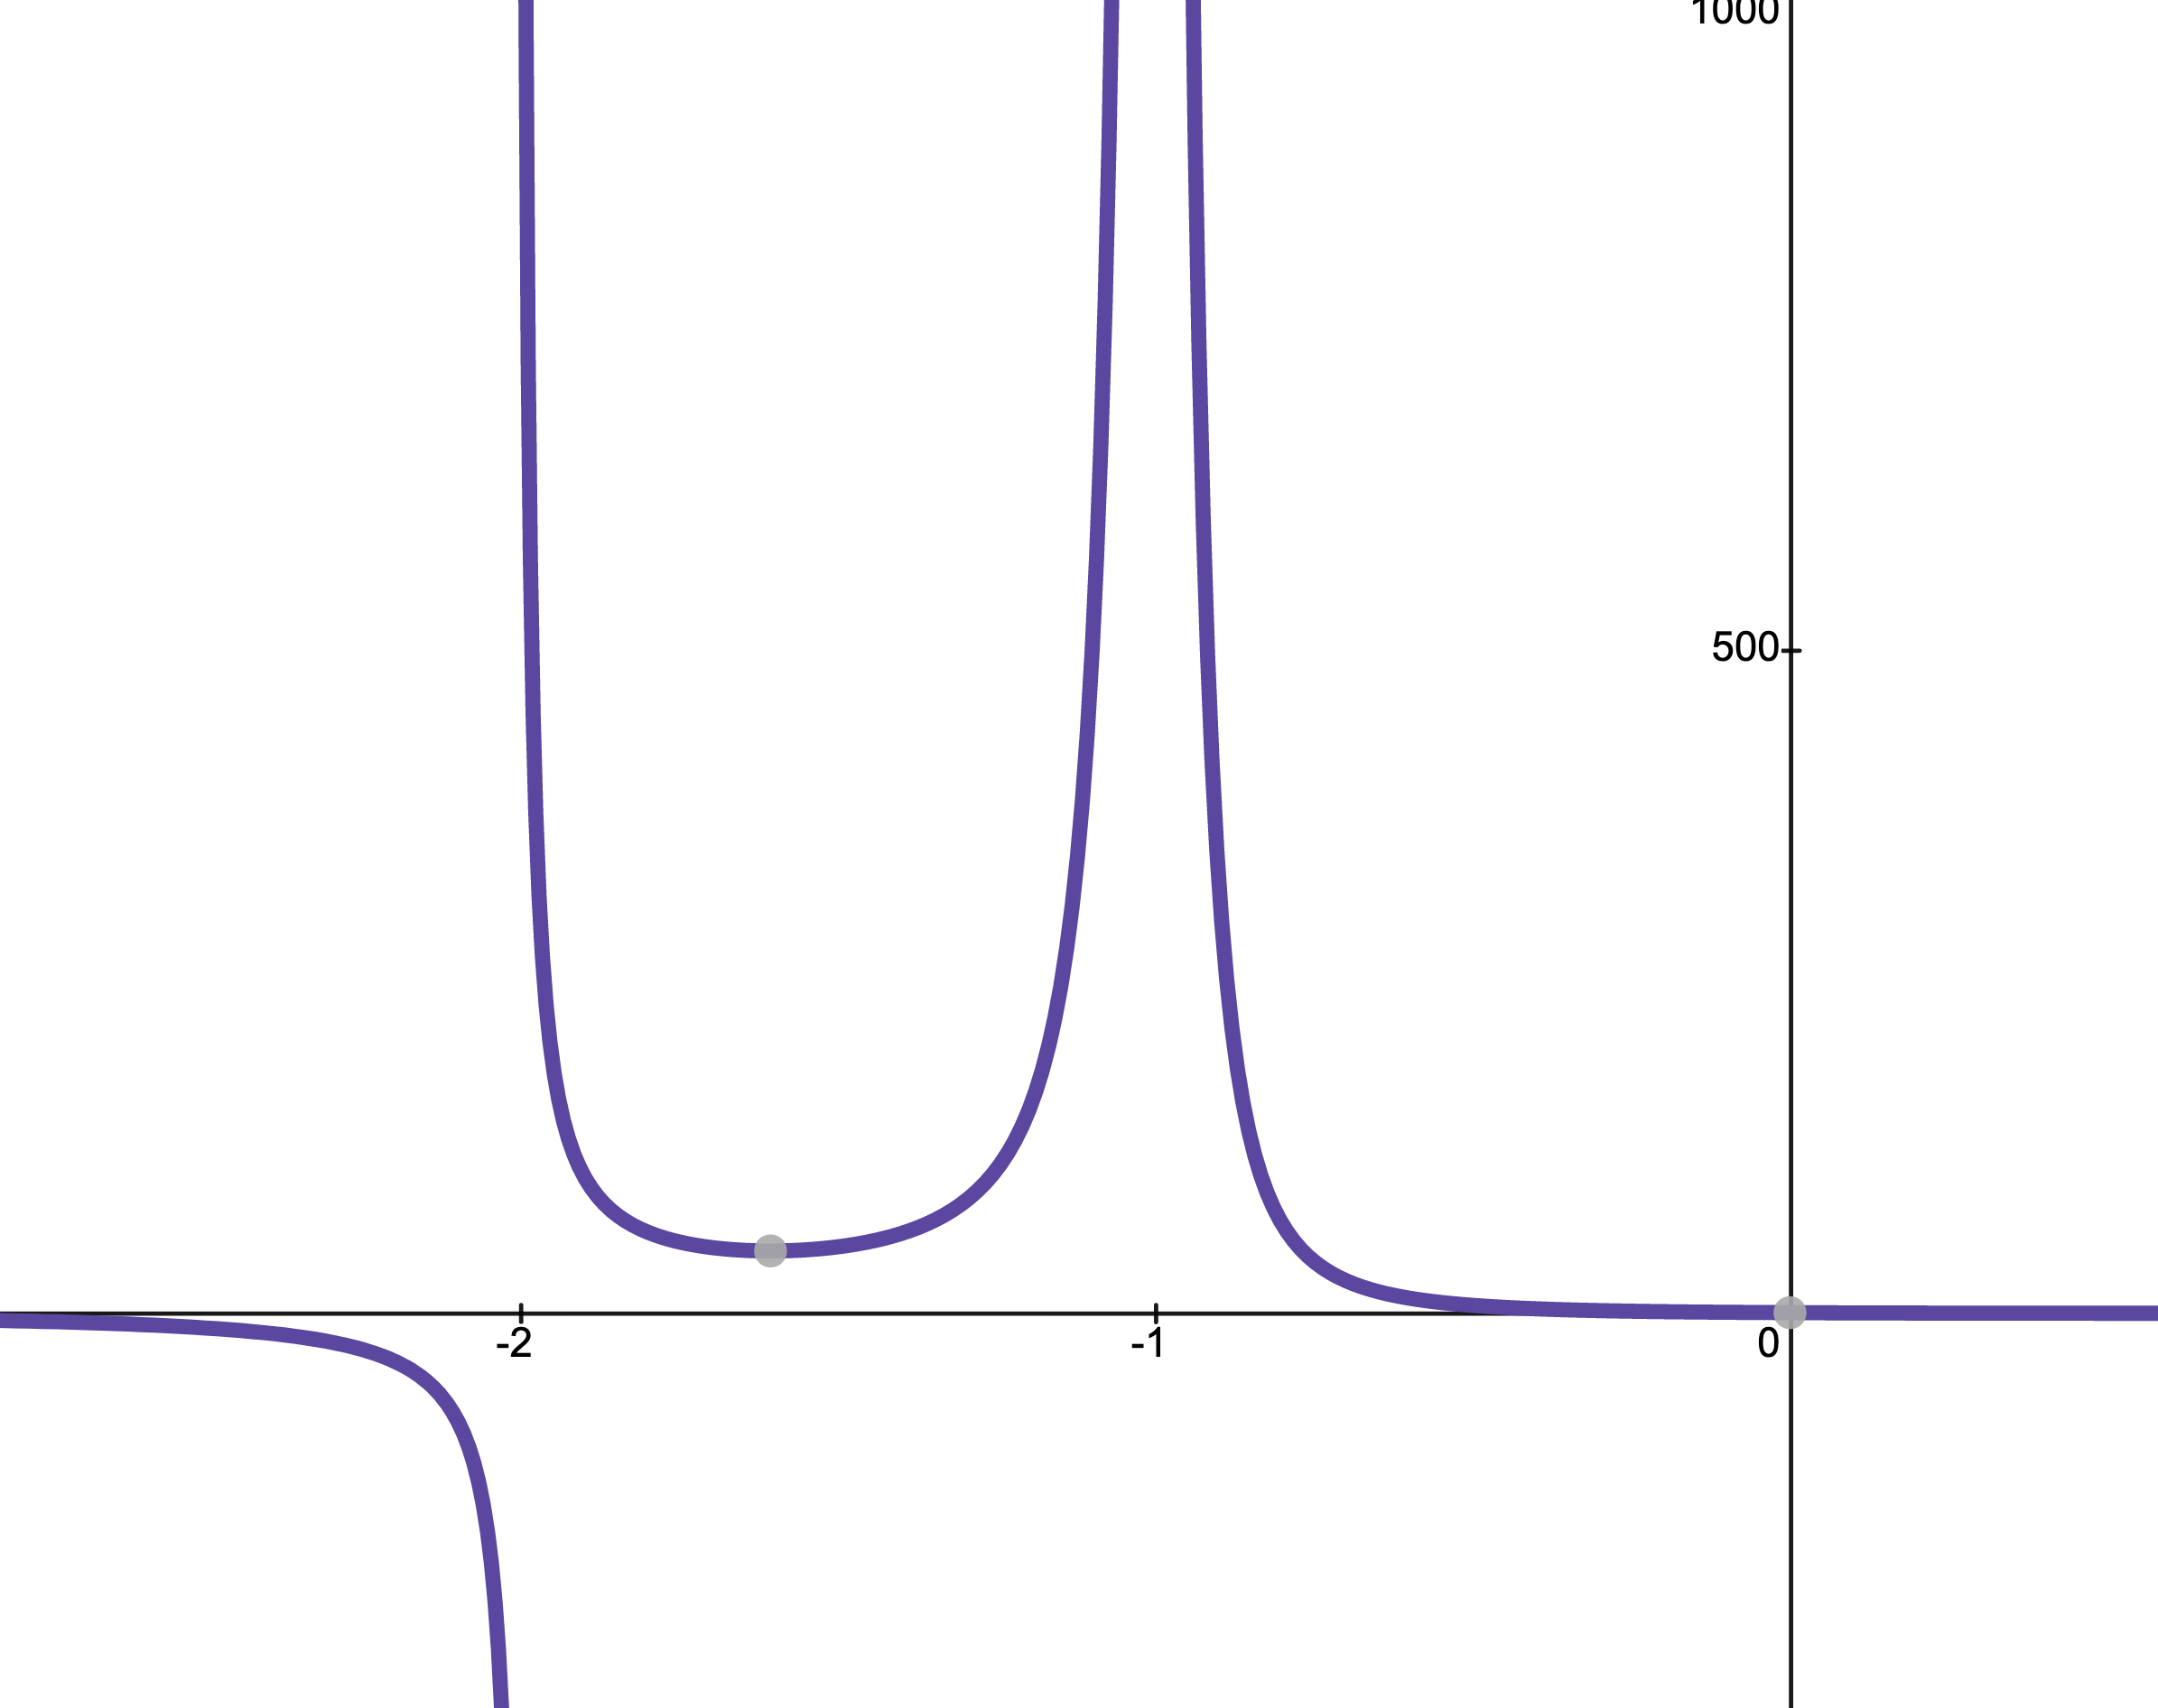
\includegraphics[height=5mm]{fig/R4}
screenshots from graphs generated using Desmos Graphing Calculator \url{https://www.desmos.com/calculator} (accessed 16 July  2021)}
\end{frame}
%----------------------------------------------------------------------------------------

%----------------------------------------------------------------------------------------
\begin{frame}[t]{Match the Function to its Graph}\AnswerNo\QuestionBar{3}{4}
A. $f(x)=|x|^e$\hfill
B. $f(x)=e^{|x|}$\hfill
C. $f(x)=e^{x^2}$\hfill
D. $f(x)=e^{x^4-x}$\vfill

\begin{multicols}{3}\centering
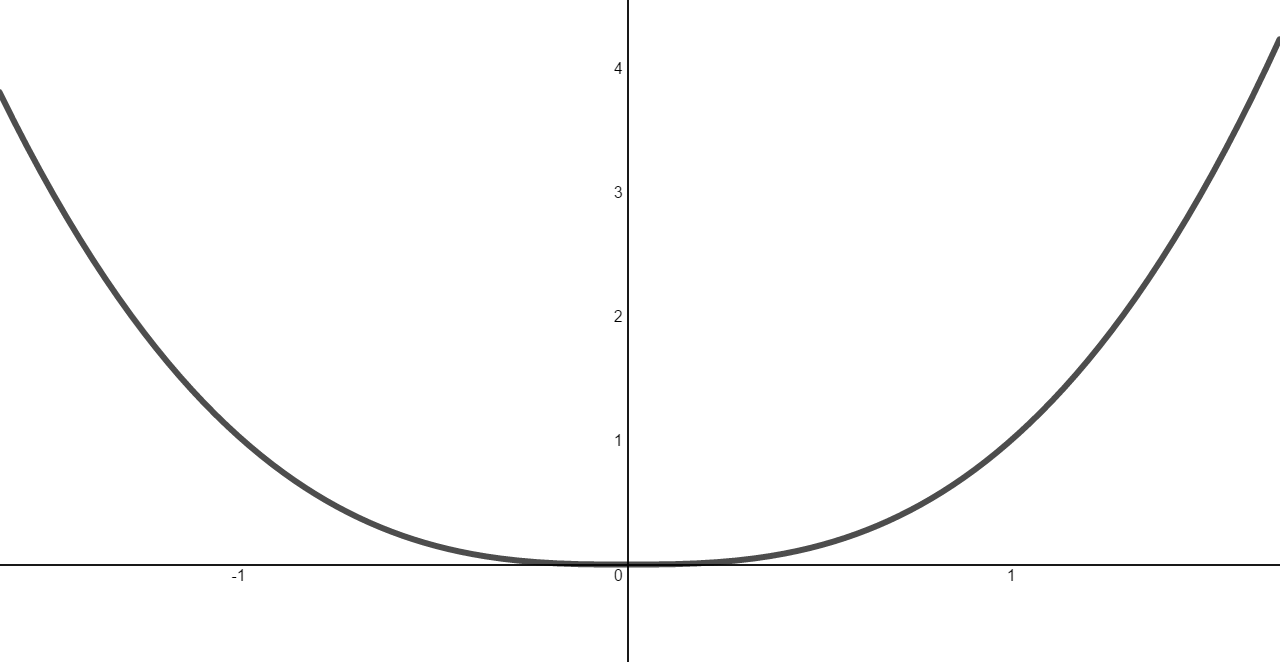
\includegraphics[width=0.33\textwidth]{fig/E1}\\
I\\[3em]

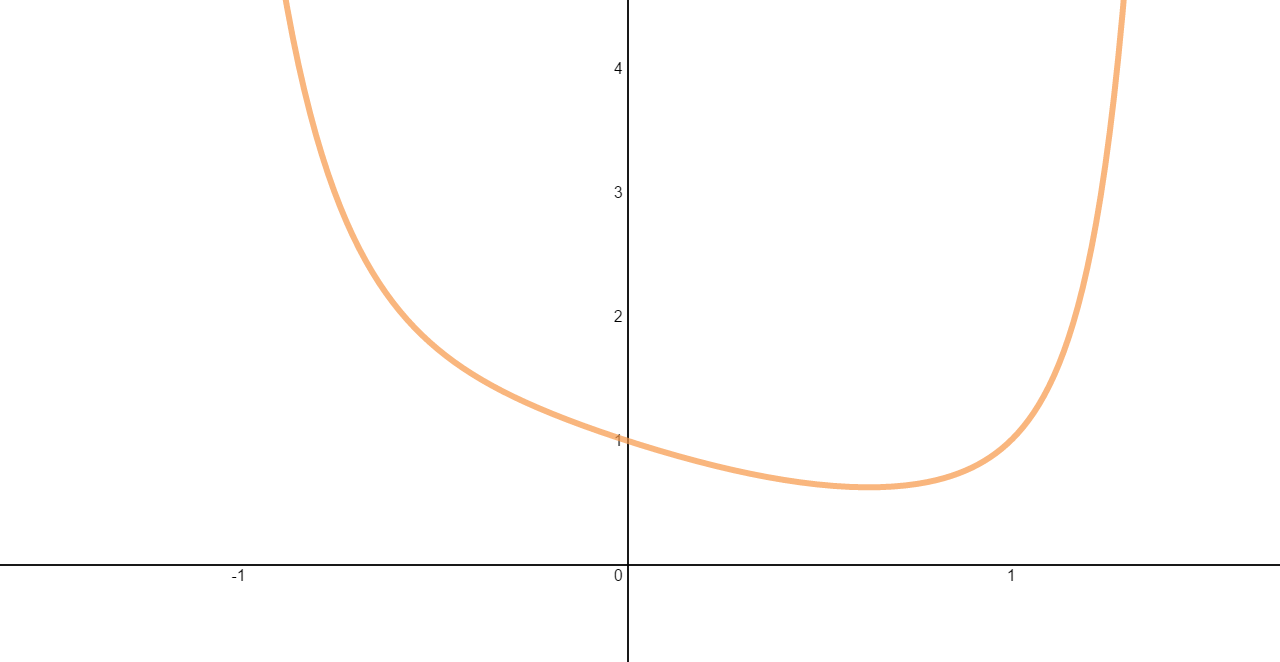
\includegraphics[width=0.33\textwidth]{fig/E2}\\
\textcolor{M5}{IV}
\columnbreak

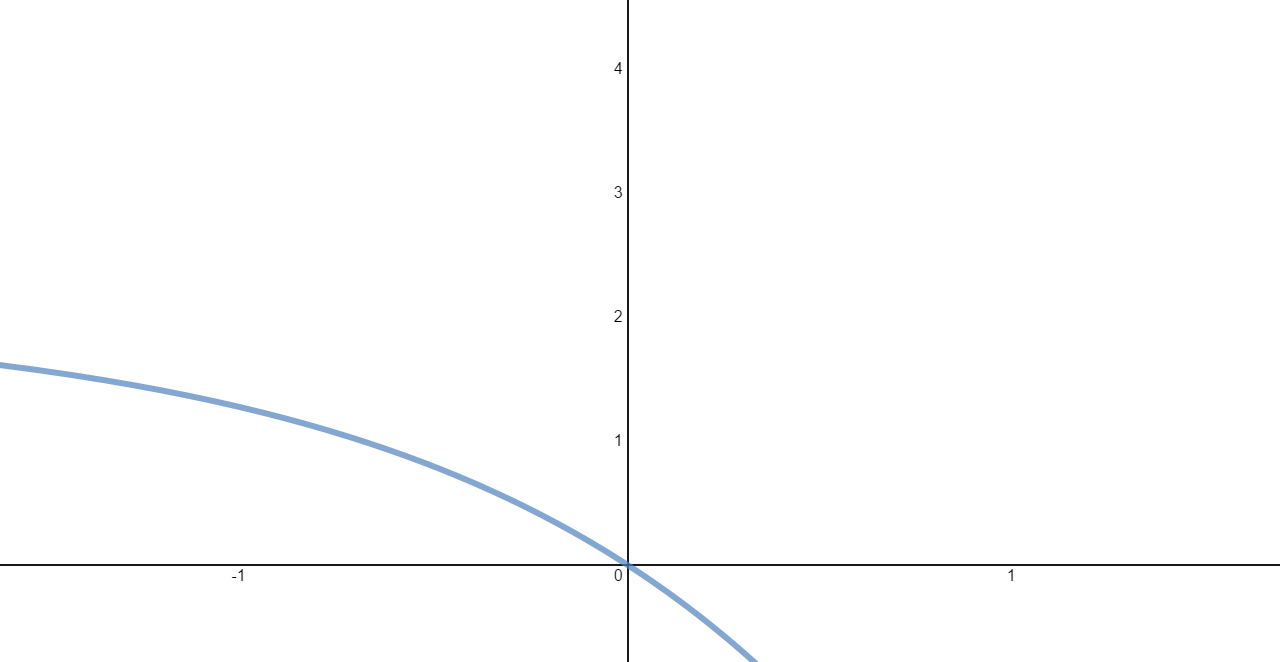
\includegraphics[width=0.33\textwidth]{fig/E6}\\
\textcolor{C4}{II}\\[3em]

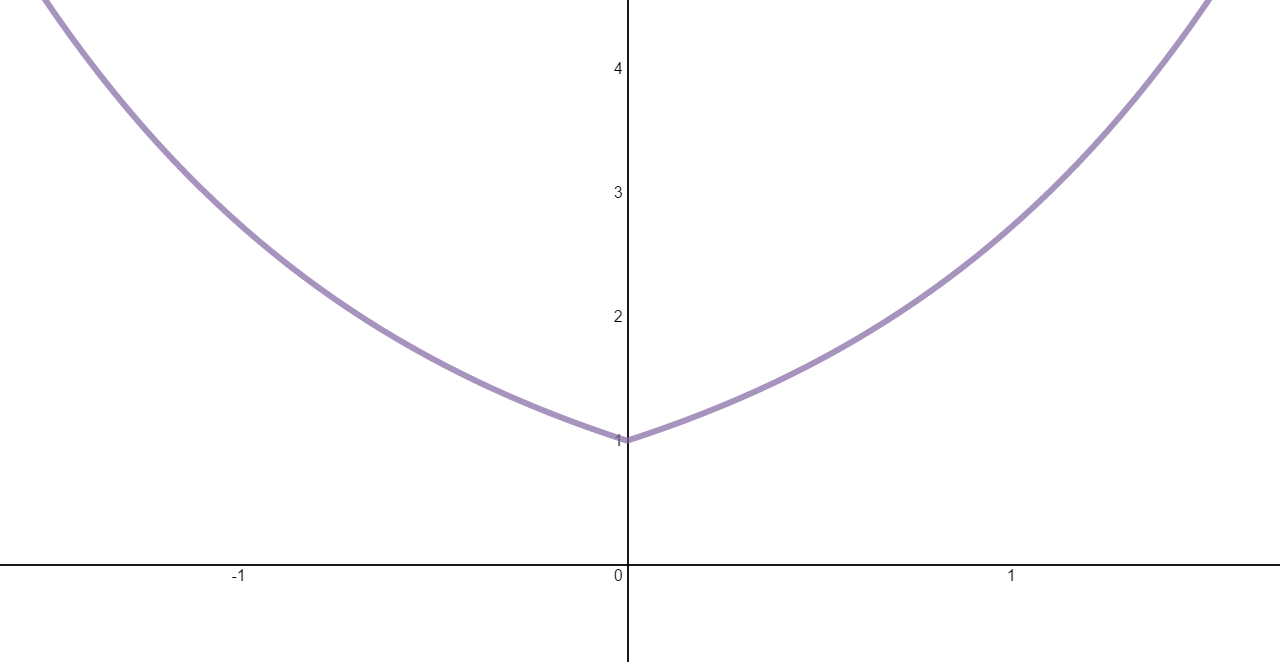
\includegraphics[width=0.33\textwidth]{fig/E3}\\
\textcolor{C3}{V}
\columnbreak

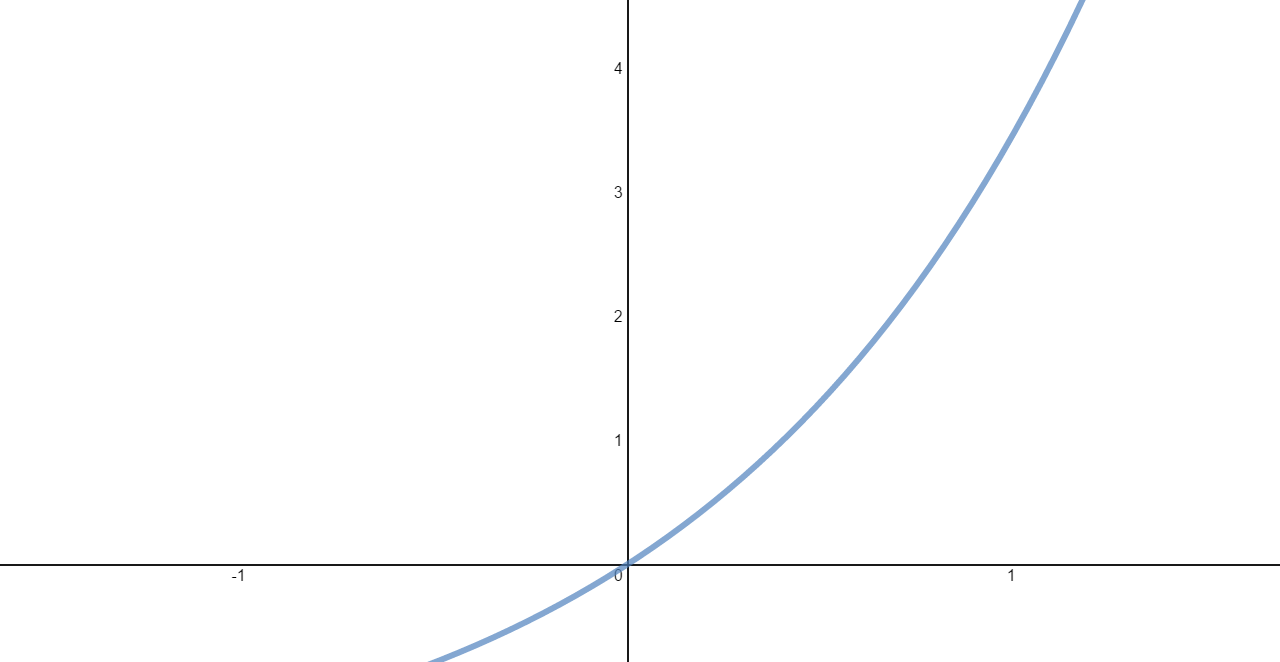
\includegraphics[width=0.33\textwidth]{fig/E5}\\
\textcolor{C1}{III}\\[3em]

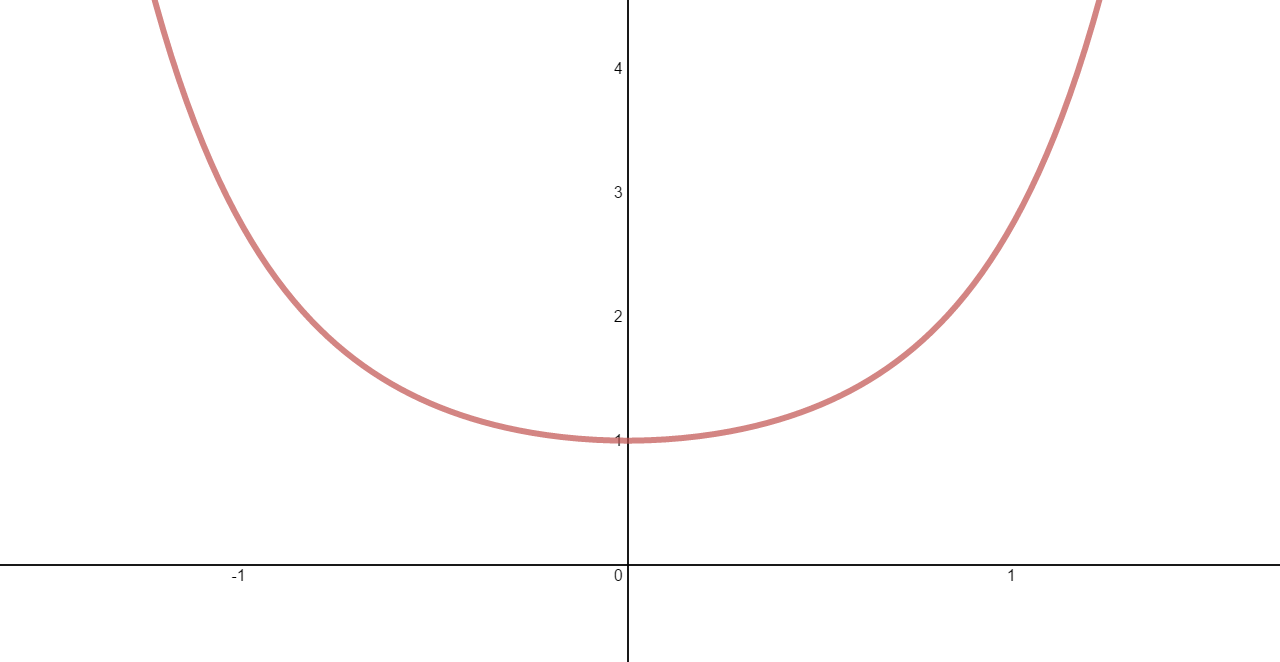
\includegraphics[width=0.33\textwidth]{fig/E4}\\
\textcolor{W1}{VI}
\end{multicols}

\index{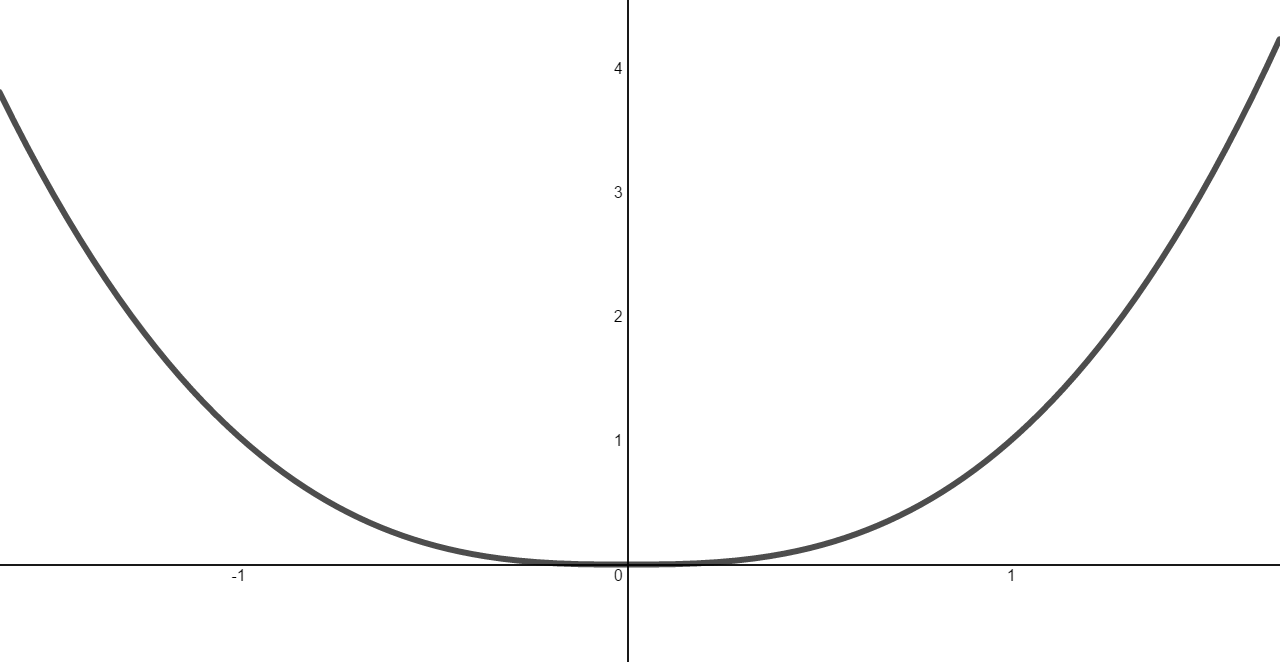
\includegraphics[height=5mm]{fig/E1},
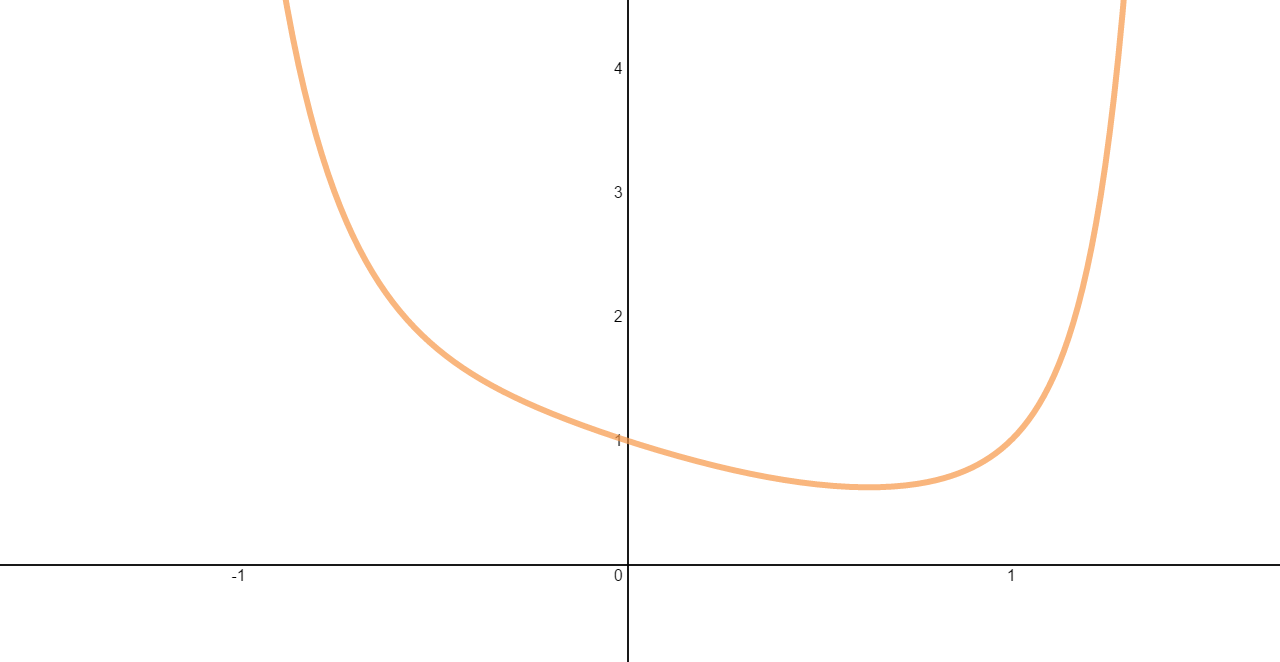
\includegraphics[height=5mm]{fig/E2},
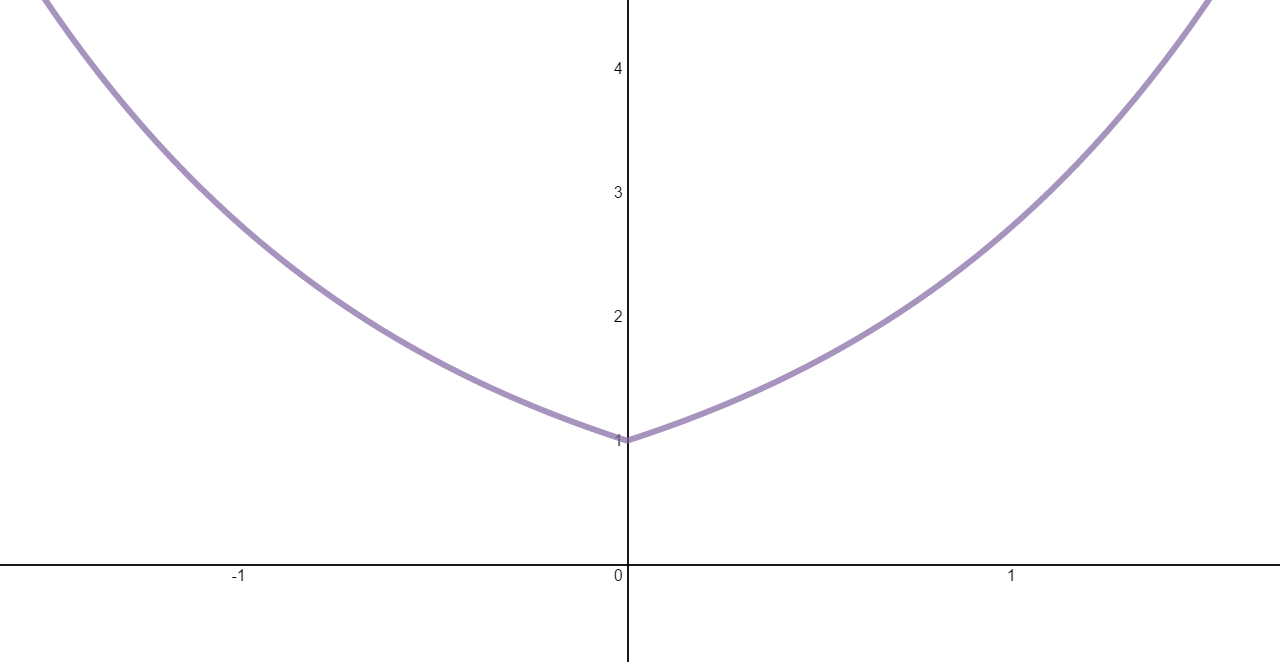
\includegraphics[height=5mm]{fig/E3},
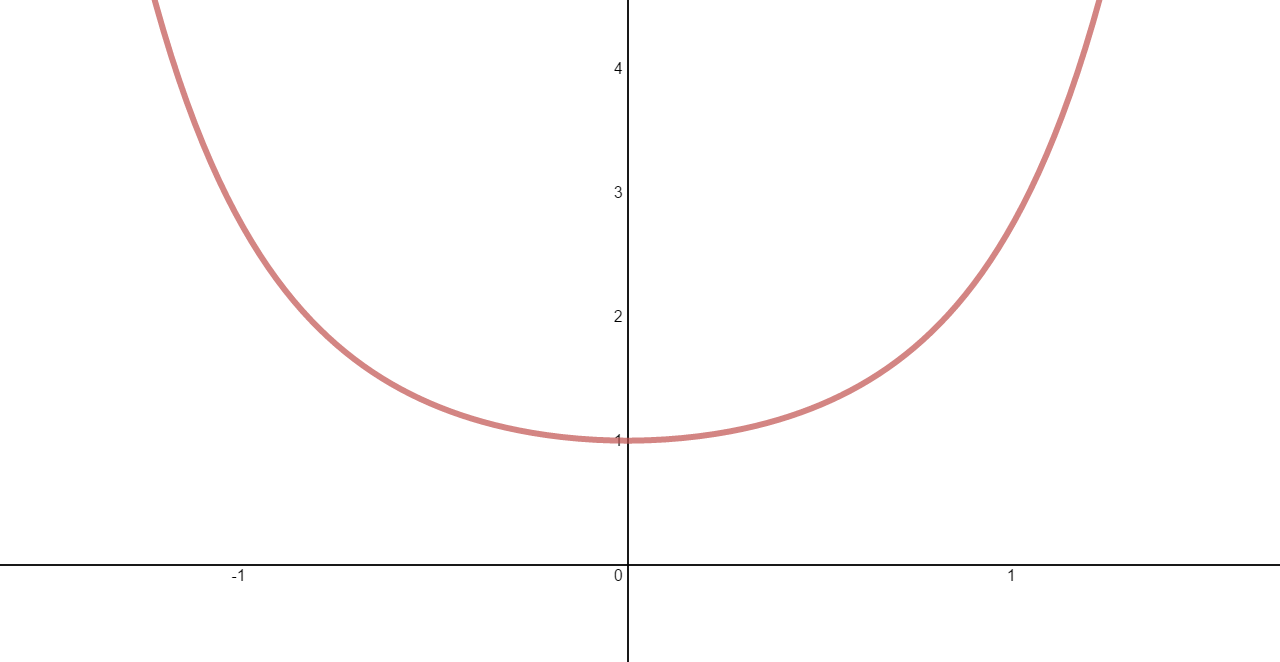
\includegraphics[height=5mm]{fig/E4},
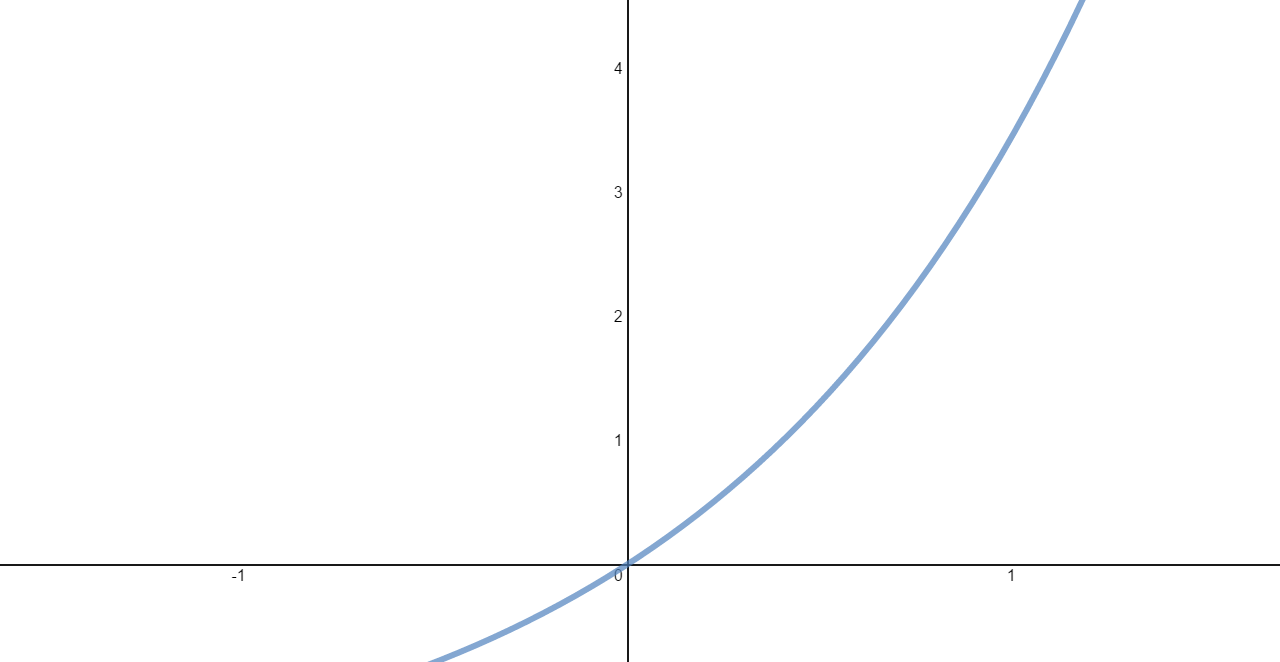
\includegraphics[height=5mm]{fig/E5},
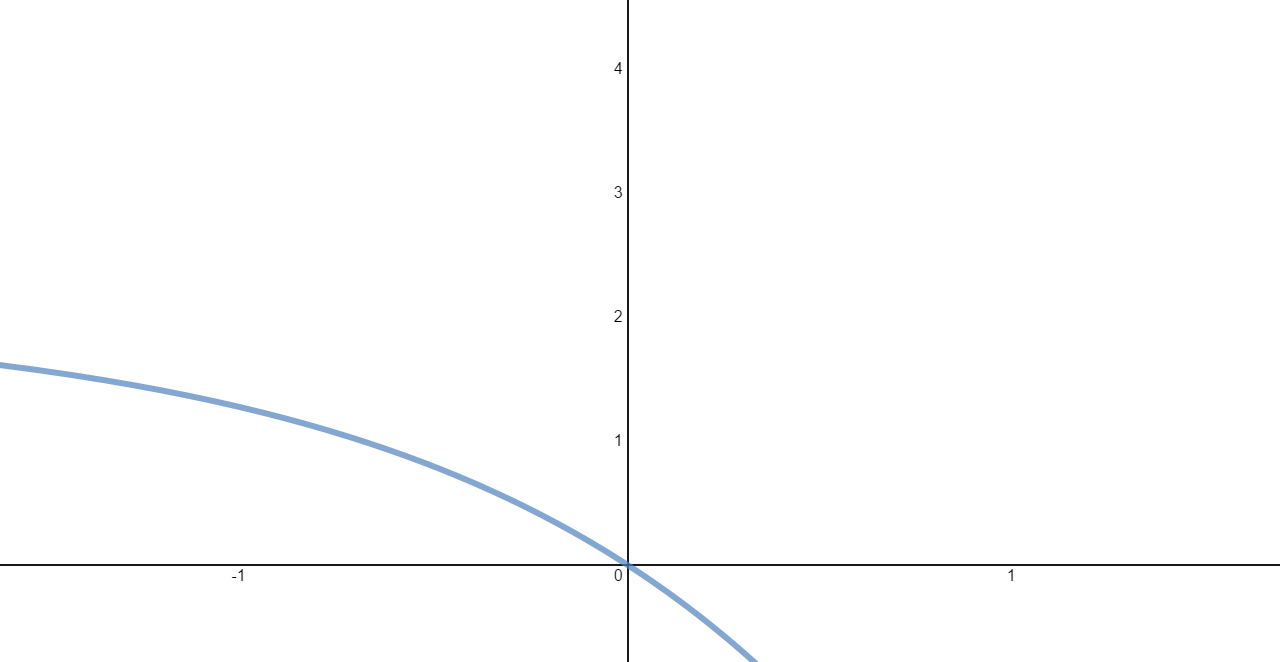
\includegraphics[height=5mm]{fig/E6}
screenshots of graphs generated using Desmos Graphing Calculator \url{https://www.desmos.com/calculator}, (accessed 13 November 2015)}

\end{frame}
%----------------------------------------------------------------------------------------
%----------------------------------------------------------------------------------------
\begin{frame}\AnswerNo\QuestionBar{4}{4}
A. $f(x)=x^5+15x^3$\hfill
B. $f(x)=x^5-15x^3$\hfill
C. $f(x)=x^5-15x^2$\\
\hfill
D. $f(x)=x^3-15x$\hfill
E. $f(x)=x^7-15x^4$\hfill~
\vfill
\centering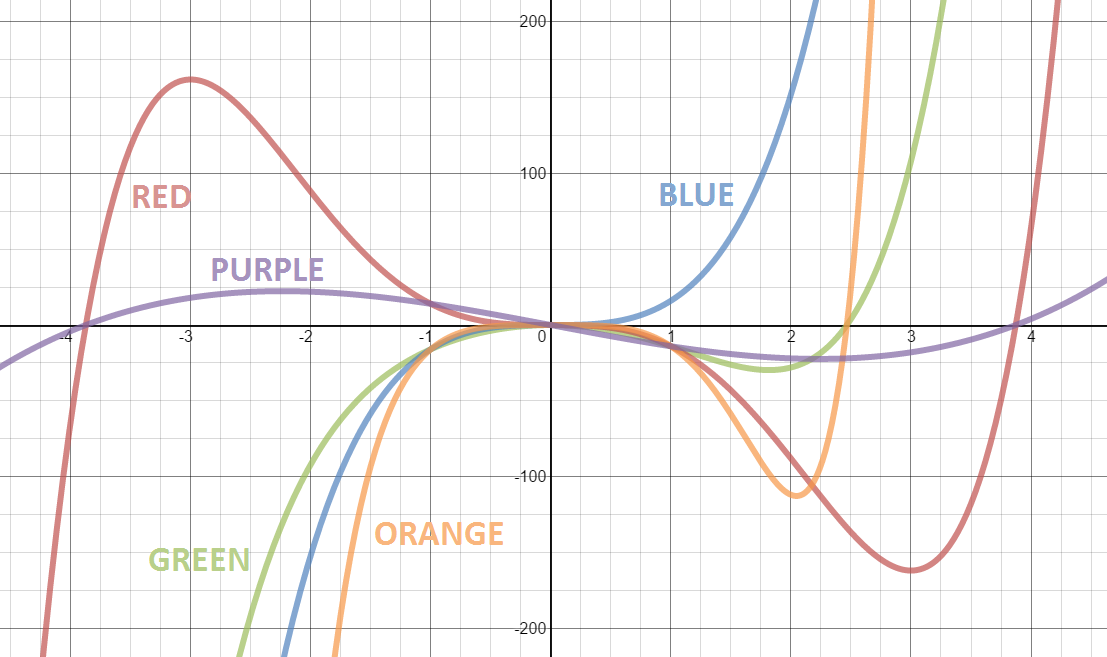
\includegraphics[width=\textwidth]{fig/polynomials}
\index{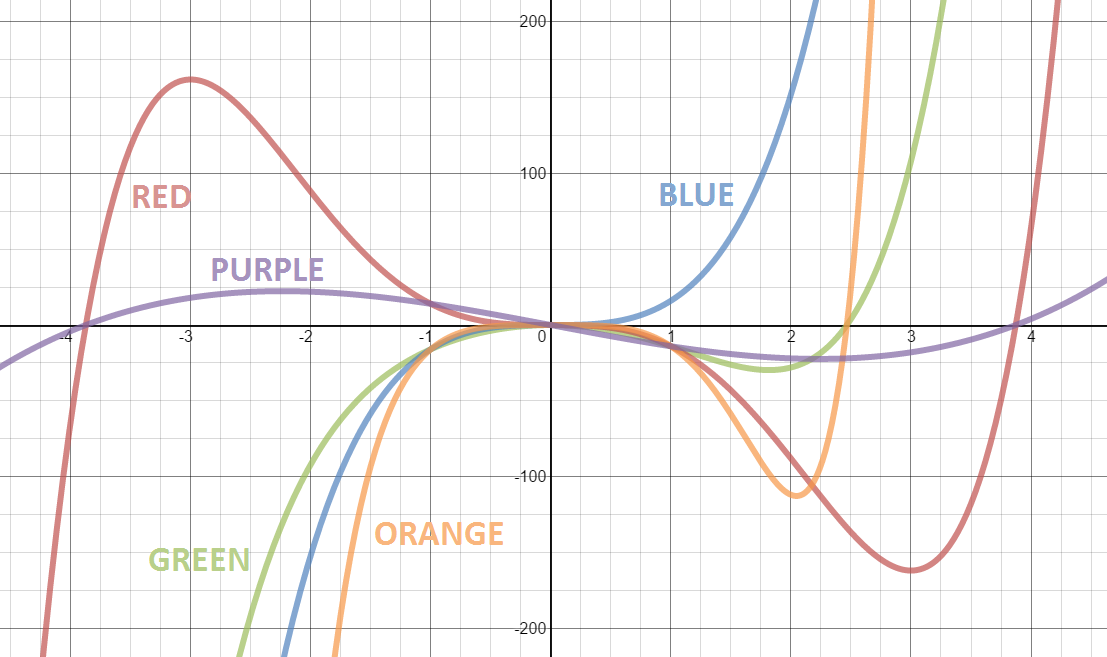
\includegraphics[height=5mm]{fig/polynomials} screenshot from graphs generated using Desmos Graphing Calculator \url{https://www.desmos.com/calculator}, with text added (accessed 13 November 2015)}
\end{frame}
%------------------------------------------------------------------
%----------------------------------------------------------------------------------------
